\part{Soft Theorem}
% 计数器清零,每个part都要引用,除了part1
\setcounter{theorem}{0}
\setcounter{definition}{0}
\setcounter{lemma}{0}
\setcounter{sidenote}{1}
\section{Review on the quantization of gravity}
本节采用\cite{Badger:2023eqz}中的记号简要回顾引力量子化以及树图顶点项。众所周知微扰量子引力是不可重整化的,所以只能看作是一个有效理论,但好就好在它的低能极限是可以用于计算引力波振幅的\cite{Goldberger:2004jt,Bern:2019crd,Mogull:2020sak}。

取自由引力场拉式量为:
\begin{equation}
	\mathcal{L}_{EH}=\frac{2}{\kappa^2}\sqrt{-g}R,\quad \kappa=\sqrt{32\pi G}
\end{equation}
然后在平直度规附近做微扰:
\begin{equation}
	g_{\mu\nu}=\eta_{\mu\nu}+\kappa h_{\mu\nu}
\end{equation}
代入到$\mathcal{L}_{EH}$进行计算得到:
\begin{equation}
	\begin{aligned}
		\mathcal{L}_{\mathrm{EH}}& =\partial_{\alpha}h\partial_{\beta}h^{\alpha\beta}-\partial_{\alpha}h_{\beta\gamma}\partial^{\beta}h^{\alpha\gamma}-\frac{1}{2}(\partial_{\alpha}h)^{2}+\frac{1}{2}(\partial_{\gamma}h_{\alpha\beta})^{2}  \\
		&+\text{total derivatives}+\mathcal{O}\left(\kappa,h^{3}\right).
	\end{aligned}
\end{equation}
其中$h\equiv h^\alpha_\alpha$。这一堆都是$(\partial h)^2$项,对应动能项,显然由于没有$h^2$项,所以引力子质量为0。后面的高阶项意味着引力子之间是有自相互作用的。

由于广义相对论是微分同胚不变的,所以他其实也是个规范理论,不同的坐标系就意味着不同的规范,度规分量的变换正对应于场的规范变换。那么我们对$h_{\mu\nu}$进行路径积分时就必须在规范下进行,这可以使用F-P鬼场方法来系统的处理。比较常用的规范选取是下面的de-Donder规范:
\begin{equation}
	G_\mu\equiv\partial^\nu h_{\mu\nu}\frac{1}{2}\partial_\mu h=0
\end{equation}
这导致规范固定项:
\begin{equation}
	{\mathcal L}_{\mathrm{GF}}=G_{\mu}G^{\mu}=\partial^{\nu}h_{\mu\nu}\partial^{\rho}h^{\mu}{}_{\rho}+\frac{1}{4}(\partial_{\mu}h)^{2}-\partial^{\nu}h_{\mu\nu}\partial^{\mu}h
\end{equation}
以及鬼场:
\begin{equation}
	\mathcal{L}_{\mathrm{GH}}=-\bar{b}^{\mu}\left(\kappa\frac{\delta G_{\mu}}{\delta\xi^{\nu}}\right)b^{\nu}
\end{equation}
de-Donder规范下:
\begin{equation}
	\kappa\frac{\delta G_{\mu}}{\delta\xi^{\nu}}=\eta_{\mu\nu}\partial^{2}+\kappa\bigl[\partial^{\rho}h_{\mu\nu}\partial_{\rho}+\partial^{\rho}h_{\nu\rho}\partial_{\mu}+\partial^{\rho}(\partial_{\nu}h_{\mu\rho})-\partial_{\mu}h_{\nu\rho}\partial^{\rho}-\frac{1}{2}\partial_{\mu}(\partial_{\nu}h)\bigr]
\end{equation}
进行路径积分时,就不必再考虑规范,取而代之$\mathcal{L}_{EH}\mapsto\mathcal{L}_{EH}+\mathcal{L}_{GF}+\mathcal{L}_{GH}$,由于树图鬼场无贡献,所以这里只考虑前两项:
\begin{equation}
	\begin{aligned}
		\mathcal{L}_{\mathrm{EH}}|_{h^{2}}+\mathcal{L}_{\mathrm{GF}}& =-\frac{1}{2}h_{\alpha\beta}\partial^{2}h_{\alpha\beta}+\frac{1}{4}h\partial^{2}h  \\
		&=-\frac{1}{2}h_{\alpha\beta}\underbrace{\left[\eta^{\alpha(\gamma}\eta^{\delta)\beta}-\frac{1}{2}\eta^{\alpha\beta}\eta^{\gamma\delta}\right]}_{I^{\alpha\beta,\gamma\delta}}\partial^{2}h_{\gamma\delta} 
	\end{aligned}
\end{equation}
给出费曼图顶点和传播子项:
\begin{equation}
	\feynmandiagram [horizontal=a to b] {a[particle=\(\alpha\beta\)] -- [gluon] b[particle=\(\gamma\delta\)]};
	=\dfrac{\text{i}P_{\alpha\beta,\gamma\delta}}{p^2-\text{i}0^+}\quad\text{with}\quad P_{\alpha\beta,\gamma\delta}=\eta_{\alpha(\gamma}\eta_{\delta)\beta}-\dfrac{1}{D-2}\eta_{\alpha\beta}\eta_{\gamma\delta}
\end{equation}
其中$I^{\alpha\beta,\gamma\delta}P_{\gamma\delta,\rho\kappa}=\delta_{(\rho}^{\alpha}\delta_{\kappa)}^{\beta}$。高阶自相互作用顶点可以在\cite{Sannan:1986tz}中找到。

引力子自旋为$2$,但由于规范的限制,其仍然如光子一样只有两个独立的极化矢量(张量),对应引力波的两种偏振模式,只不过这个时候其实是个二阶对称极化张量。满足下面的条件:
\begin{equation} 
	p_\mu \epsilon^{\mu\nu}_{++/--} (p)=0,\quad \eta_{\mu\nu} \epsilon^{\mu\nu}_{++/--} (p)=0
\end{equation}
利用光子的极化矢量,可以构造出一组非常方便的$\epsilon^{\mu\nu}_{++/--}$选取:
\begin{equation}
	\epsilon^{\mu\nu}_{\pm\pm}=\epsilon^{\mu}_{\pm}\epsilon^{\nu}_{\pm}
\end{equation}

现在考虑引力场与其他场的耦合,耦合项拉式量为:
\begin{equation}
	\mathcal{L}_{\text{int}}=\frac{\kappa}{2}h^{\mu\nu}T_{\mu\nu}
\end{equation}
这里$T_{\mu\nu}$是场的能动张量,可以使用下式进行计算:\sn{平直时空中能动量张量是根据Poincar\'e不变性引入的Noether current,可以说明(见\ref{eq:19.8})实际上等价于$$\left.T_{\mu\nu}\right|_{\text{flat}}=-2\left.\frac{\delta S_M}{\delta g^{\mu\nu}}\right|_{g^{\mu\nu}=\eta_{\mu\nu}}$$GR里面的能动量张量就是这个的推广。}
\begin{equation}
	T_{\mu\nu}(x)=-\frac{2}{\sqrt{-g}}\frac{\delta S_M}{\delta g_{\mu\nu}(x)}
\end{equation}
$S_M$是物质场的作用量,但是是在弯曲时空中的,可以使用最小耦合方法得到\sn{玻色场可以这么做,费米场复杂些}。以自旋为0对应的实标量场为例。
\begin{equation}\label{S_M}
	S_M=\int d^4x\sqrt{-\eta}\left(-\frac{1}{2}\eta^{\mu\nu}\partial_\mu\phi\partial_\nu\phi-V(\phi)\right)
\end{equation}
这里我们把所有暗含$\eta$的地方都显式的写出来了,弯曲时空中的作用量只需要将$\eta\mapsto g,\partial\mapsto\nabla$即可,得到:
\begin{equation}
	\tilde S_M=\int d^4x\sqrt{-g}\left(-\frac{1}{2}g^{\mu\nu}\nabla_\mu\phi\nabla_\nu\phi-V(\phi)\right)
\end{equation}

当然,对称性允许我们在后面添加正比于Ricci标量的项等等,但所谓我们要的就是“最小”耦合。不过在微扰引力框架下,我们其实只需要利用\ref{S_M}对$\eta$求变分导数就好了,对于无质量的自由标量场(对应不动点处的理论),我们得到\sn{实际上,考虑弯曲背景时空之后,多出了一些可重整的项可以加入到作用量中,比如$R\phi$,对于平直时空$R=0$,这一项不用考虑}:
\begin{equation}\label{eq:20.10}
	T_{\mu\nu}=\partial_\mu\phi\partial_\nu\phi-\frac{1}{2}\eta_{\mu\nu}\partial^\rho\phi\partial_\rho\phi
\end{equation}
对应的顶点项为:
\begin{equation}
	\feynmandiagram [inline=(d.base), horizontal=d to b] {
		a --[momentum=\(p\)]  b[dot] --[momentum=\(q\)]  c,
		b -- [gluon] d ,
	};
	= i \kappa p_{\mu}q_\nu +\text{正比于}\eta_{\mu\nu}\text{的项}
\end{equation}

\section{Soft theorem from feynman diagrams}
所谓软粒子,指的就是动量趋于0的无质量粒子,因为无质量$E=cp$,所以能量也会趋于0,任意过程都会辐射出期望值为无限多个的软粒子。本节使用费曼图方法讨论辐射软粒子的振幅修正\cite{McLoughlin:2022ljp}。

首先考虑辐射一个软光子,理论背景为旋量QED,散射过程为$ne^-\to me^-+\gamma $,注意考虑的是一般的旋量QED,可以有不同味的电子,电荷为$Q_i$。这里考虑的是电子,正电子的讨论也类似,最终结论是一样的。

辐射软光子可以从入射外线辐射,也可以从出射外线辐射,还可以从内线辐射:
\begin{figure}[H]
	\centering
	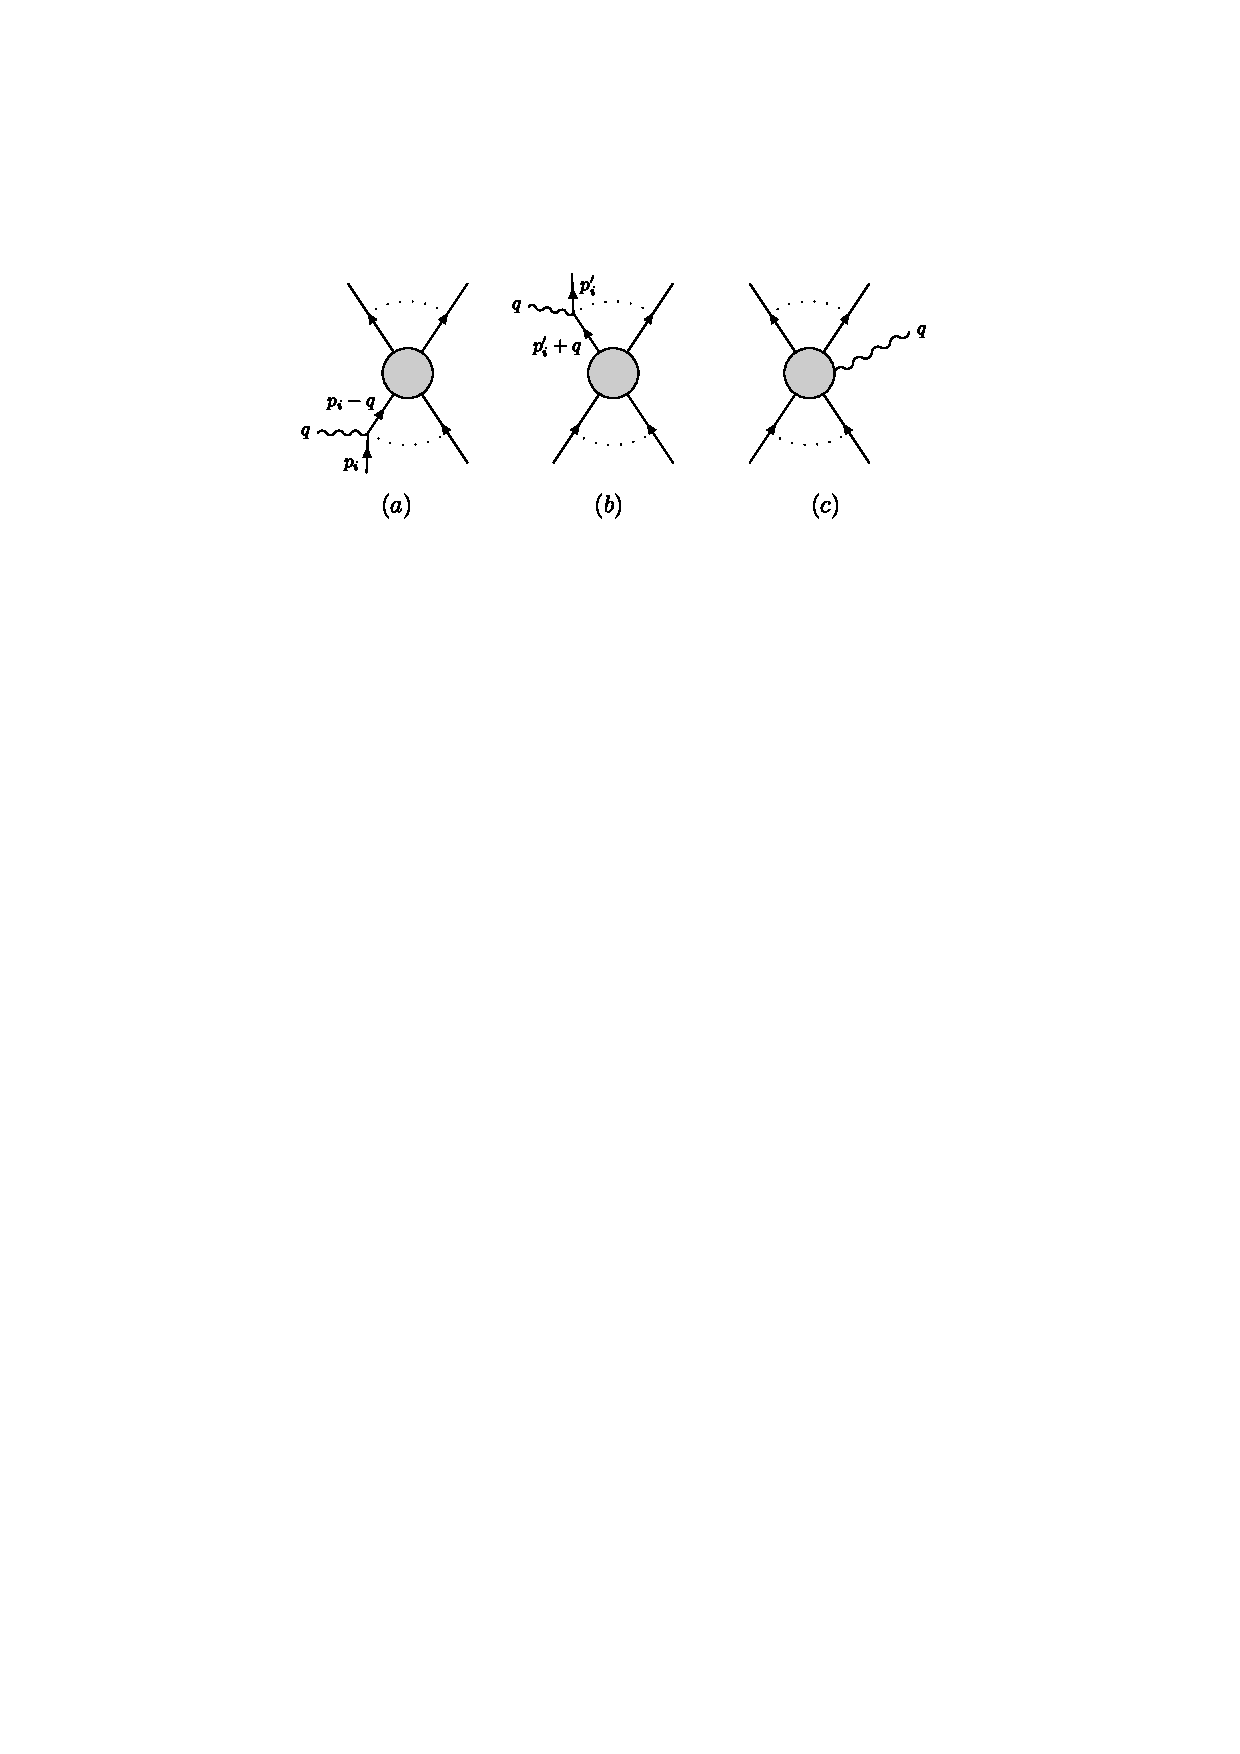
\includegraphics[width=0.8\linewidth]{figs/fig3.pdf}
	\caption{辐射软光子的三种情况}
\end{figure}
我们使用$\mathcal{A}(p,q)$表示辐射一个软光子后的振幅$\mathcal{A}(p)$表示没有辐射软光子的振幅(所有阶费曼图求和)。用$T(p_i-q)$表示原先没有辐射软光子的费曼图砍掉一个$p_i$外线但保留外线动量为非在壳的$p_i-q$得到的费曼图振幅,显然$T(p_i)u(p_i)=\mathcal{A}(p)$。

首先计算入射外线辐射软光子:
\begin{equation}
	\begin{aligned}
		Q_iT(p_i-q)\frac{(-\slashed{p}_i^\prime+\slashed{q}+m)\slashed{\epsilon}(q)}{(p_i-q)^2+m^2}u(p_i)&=-Q_iT(p_i-q)\Big[\frac{\epsilon(q)\cdot p_i+i\epsilon(q)_\mu q_\nu S^{\mu\nu}}{q\cdot p_i+\mathrm{i}0^+}\Big]u(p_i)
	\end{aligned}
\end{equation}
其中利用了$\slashed{a}\slashed{b}=-2a\cdot b-\slashed{b}\slashed{a}$,$q\cdot \epsilon_\pm(q)=0$以及狄拉克方程$(\slashed{p}+m)u(p)=0$。其中$S^{\mu\nu}=\frac{\mathrm{i}}{4}[\gamma^\mu,\gamma^\nu]$。唯一做近似的地方就是分母里面的$q^2$我们略去了,这对后面的高阶修正也不会影响。这一注意到$q=0$实际上是一个极点,这是因为在光子无线“软”的时候,多出来的那条内线传播子会无线趋于在壳,导致分母为0。

对于出射粒子辐射软光子也是类似的计算得到:
\begin{equation}\label{eq:20.17}
	\begin{aligned}
		Q^\prime_i\bar u(p_i^\prime)\frac{(-\slashed{p}_i^\prime-\slashed{q}+m)\slashed{\epsilon}(q)}{(p_i-q)^2+m^2}\bar T(p_i+q)&=Q^\prime_i\bar u(p_i^\prime)\Big[\frac{\epsilon(q)\cdot p_i+i\epsilon(q)_\mu q_\nu S^{\mu\nu}}{q\cdot p_i-\mathrm{i}0^+}\Big]\bar T(p_i-q)
	\end{aligned}
\end{equation}

至于内线发射光子,我们用$N^\mu(p,q)$表示,而且注意到$q\to0$时$N$非奇异,而且内线本身就是不在壳的,所以可以认为$N^\mu(p,q)\sim\mathcal{O}(q^0)$。三项加起来得到:
\begin{equation}\label{eq:21.3}
	\begin{aligned}
		\mathcal{A}(p,p^{\prime},q) =&\sum_\text{incoming }{ - Q _ i T ( p _ i - q )}\frac{\epsilon(q)\cdot p_i+i\epsilon(q)_{\mu}q_\nu S^{\mu\nu}}{q\cdot p_i+\mathrm{i}0^+}u(p_i)  \\
		&+\sum_{\mathrm{outgoing}}Q_{i}^{\prime}\bar{u}(p_{i}^{\prime})\frac{\epsilon(q)\cdot p_{i}^{\prime}+i\epsilon(q)_{\mu}q_{\nu}{S}^{\mu\nu}}{q\cdot p_{i}^{\prime}-\mathrm{i}0^+}\bar{T}(p_{i}^{\prime}+q)\\
		&+\epsilon(q)_{\mu}N^{\mu}(p,p^{\prime},q)
	\end{aligned}
\end{equation}
考虑最低阶修正,也就是只保留极点,得到:
\begin{equation}\label{eq:21.4}
	\boxed{
	\mathcal{A}(p,q)=\left[\sum_{i}\eta_iQ_{i}\frac{\epsilon(q)\cdot p_{i}}{q\cdot p_{i}}\right]\mathcal{A}(p)}+\mathcal{O}(1)
\end{equation}
其中对于入射粒子$\eta_i=-1$,出射粒子为$+1$。QED中辐射出光子的振幅都可以拆分成$\epsilon(q)_\mu \mathcal{M}^\mu$,振幅是相对论不变量,但是我们虽然常说$\epsilon(q)_\mu$是极化矢量,但它并不是真正意义上的矢量,因为其在lorentz变换下并不协变,而是会多出来一个正比于$q$的项\sn{我们是在Lorentz变换的意义下理解,其实矢量的这种变换完全可以理解为规范选取不同,从而从振幅的规范不变性导出结果。\cite{srednicki}}\cite{Weinberg}。为了让振幅是相对论不变量,必须有:
\begin{equation}\label{eq:21.5}
	\boxed{
	q_\mu\mathcal{M}^\mu=0}
\end{equation}
也就是Ward恒等式,也可以从Ward-高桥恒等式在U(1)对称性下导出它,实际上也就是利用电荷守恒导出它,但是前面我们的导出仅仅依赖于Lorentz不变性。现在把\ref{eq:21.4}中的$\epsilon(q)$替换为$q$我们得到:
\begin{equation}\label{eq:21.6}
	\left[\sum_i\eta_i Q_i\right]\mathcal{A}(p)=0
\end{equation}
也就是说,如果散射过程不被禁闭,也就是$\mathcal{A}(p)\neq 0$,那么这个过程必然要电荷守恒!另外说一句,我们这里的推导得到的\ref{eq:21.4}对于任意自旋的场都适用,比如对于标量QED,只需要把$S^{\mu\nu}$替换为0就好,不同的自旋对应$S^{\mu\nu}$的不同表示。

现在继续考虑两个光子的情况,两个光子由不同外线发射,在最低阶近似下只是乘上了\ref{eq:21.4}中两个因子,但是由相同外线发射就要考虑发射的先后顺序,因子形式会变化:
\begin{figure}[H]
	\centering
	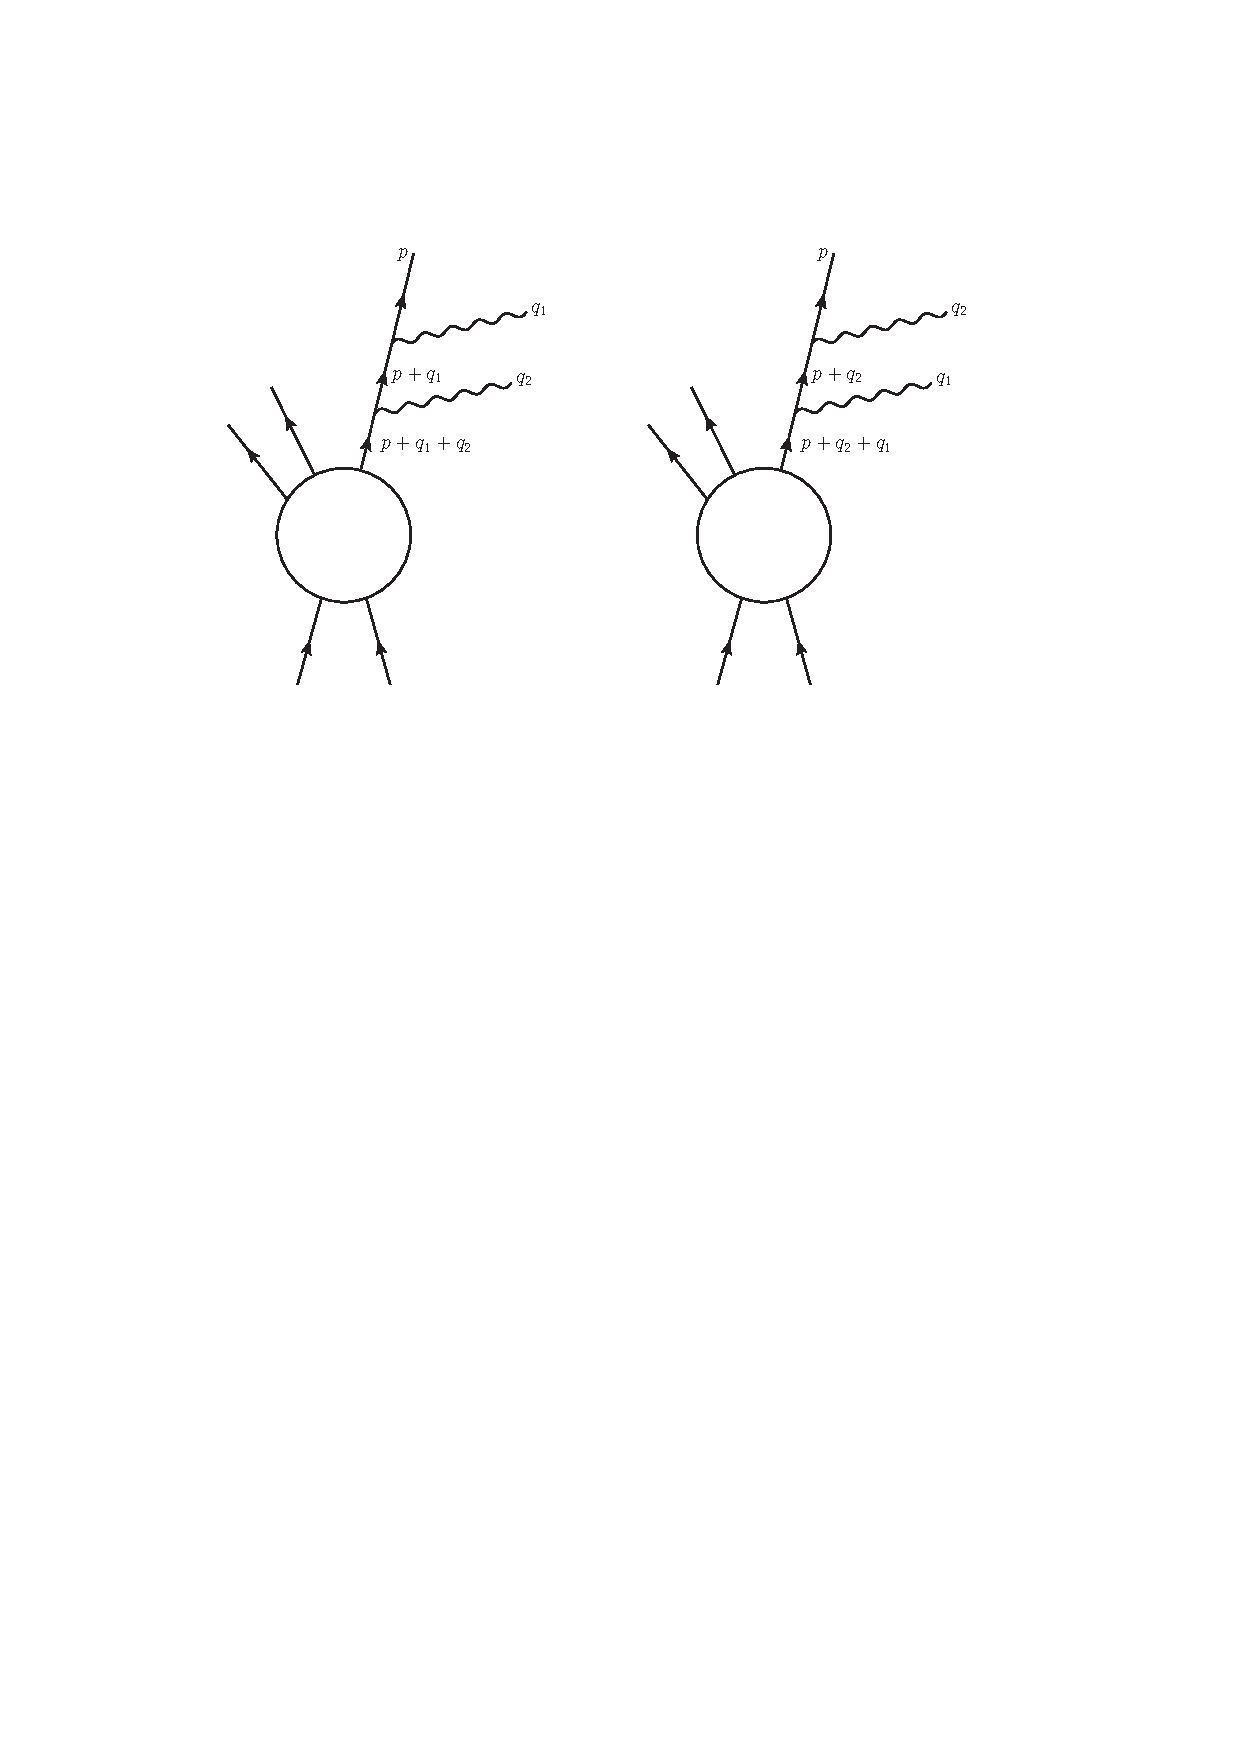
\includegraphics[width=0.8\linewidth]{figs/fig4.pdf}
	\caption{同一外线辐射两个软光子}
\end{figure}
把两幅图贡献的因子加起来得到:
\begin{equation}
	\begin{aligned}
	&\left[\frac{\eta Q\epsilon(q_1)\cdot p}{p\cdot q_1-\mathrm{i}\eta0^+}\right]\left[\frac{\eta Q\epsilon(q_2)\cdot p}{p\cdot(q_2+q_1)-\mathrm{i}\eta 0^+}\right]+\left[\frac{\eta Q\epsilon(q_2)\cdot p}{p\cdot q_2-\mathrm{i}\eta0^+}\right]\left[\frac{\eta Q\epsilon(q_1)\cdot p}{p\cdot(q_1+q_2)-\mathrm{i}\eta 0^+}\right]\\=&\left[\frac{\eta Q\epsilon(q_1)\cdot p}{p\cdot q_1-\mathrm{i}\eta0^+}\right]\left[\frac{\eta Q\epsilon(q_2)\cdot p}{p\cdot q_2-\mathrm{i}\eta 0^+}\right]	
	\end{aligned}
\end{equation}
得到的结果就是不同外腿上面的辐射两个软光子得到的因子,利用数学归纳法可以证明这一结论对于辐射任意数量的软光子都是适用的,那么最终我们只需要把因子乘起来,然后对所有外腿求和就好了,用式子表示如下:
\begin{equation}
	\boxed{\mathcal{A}(p,q_1,\ldots,q_m)=\prod_{j=1}^m\left[\sum_{i=1}^nQ_i\eta_i\frac{\epsilon(q_j)\cdot p_i}{q_j\cdot p_i}\right]\mathcal{A}(p)++\mathcal{O}(1)}
\end{equation}
前面的因子称为\textbf{eikonal因子}。推广到non-Abelian Y-M场的软定理也早有人计算过了\cite{Berends:1987me,Berends:1988zn,Mangano:1987kp,Mangano:1990by},软定理更多更一般的推广见\cite{McLoughlin:2022ljp}的文献索引。

现在来考虑辐射一个软引力子的情况,考虑第一节引入的标量场模型,传播子为:
\begin{equation}
	-\frac{i }{(p+\eta q)^2+m^2}
\end{equation}
顶点由\ref{eq:20.17}给出,但是由于\ref{eq:20.10},要与$\epsilon^{\mu\nu}$缩并,正比于$\eta_{\mu\nu}$的项没有贡献。以出射外线辐射软引力子为例,给出因子:
\begin{equation}
	i\sqrt{32\pi G}\varepsilon^{\mu\nu}p_{\mu}p_{\nu}\frac{-i}{\left(p+q\right)^{2}+m^{2}}\rightarrow\sqrt{8\pi G}\frac{\varepsilon^{\mu\nu}p_{\mu}p_{\nu}}{p\cdot q}
\end{equation}
求和后得到:
\begin{equation}
	\boxed{
	\mathcal{A}(p,q)=\left[\sum_i\frac{\kappa_i}{2}\eta_i\frac{\epsilon_{\mu\nu}(q)p_i^\mu p_i^\nu}{q\cdot p_i}\right]\mathcal{A}(p)+\mathcal{O}(1)}
\end{equation}

引力子同样有类似于\ref{eq:21.5}的恒等式,由此我们可以得到所有的$\kappa_i$都是相等的\sn{这里有点循环论证了,因为前面为了推导的方便我们同一取$\kappa_i=\sqrt{32\pi G}$},也就是等效原理!而自旋大于二的软粒子的软定理沿用上面的方法给出的限制就太强了,以至于散射$\mathcal{S}$矩阵必须trivial,所以一般认为自旋大于二的无质量粒子在“变软”的时候就脱耦合了。
\section{Subleading and subsubleading order soft theorem}
考虑动量为$\delta q,\delta \to0$的软光子辐射,$\pm$表示软光子的螺旋度,而$\ell_i$表示其它粒子的螺旋度,则更一般的软定理可以用洛朗展开写成:
\begin{equation}
	\mathcal{A}_{\ell_1,...,\ell_n,\pm}(p,\delta q)=\left[\sum_{a=0}^\infty\delta^{-1+a}S_\pm^{(a)}\right]\mathcal{A}_{\ell_1,...,\ell_n}(p)
\end{equation}
次领头阶的计算可以从\ref{eq:21.5}式出发,将\ref{eq:21.3}中所有的$\epsilon$替换为动量,保留到$\mathcal{O}(\delta^0)$,并且令等式左边为0。注意到这一阶近似下可以有$N^\mu(p,q)\approx N^\mu(p,0)$,得到:
\begin{equation}
	-q^{\mu}N_{\mu}(p,0)=\cancelto{0}{\frac{1}{\delta}\sum_{i=1}^{n}\eta_{i}Q_{i}\mathcal{A}(p)}+q^{\mu}\sum_{i=1}^{n}Q_{i}\frac{\partial}{\partial p_{i}^{\mu}}\mathcal{A}(p)
\end{equation}
其中第一项为0是因为电荷守恒\ref{eq:21.6},第二项中的$\partial_{p_i}$只作用于$\mathcal{A}$中的$T$,不作用于$u$\sn{因为这个式子的导出,是对$T(p\pm q)$展开得到的。}。这样就确定出了$N^\mu$\sn{其实只能确定到某个与$q$无关的矢量$v$,满足$q\cdot v=0$,但是这样的$v$实际上不存在。},再带回到\ref{eq:21.3}得到:
\begin{equation}
	A^\mu=\sum_{i=1}^nQ_i\left[\frac{\eta_ip_i^\mu}{\delta q\cdot p_i}+\frac{q^\nu p_i^\mu}{q\cdot p_i}\frac{\partial}{\partial p_i^\nu}-\frac{iq_\nu S_i^{\mu\nu}}{q\cdot p_i}-\frac{\partial}{\partial p_{i\mu}}\right]\mathcal{A}(p)+\mathcal{O}(\delta)
\end{equation}
这个式子里面的$\partial_{p_i}$就是作用于整个$\mathcal{A}$了。定义:
\begin{equation}
	L_i^{\mu\nu}=i\left(p_i^\mu\frac{\partial}{\partial p_{i\nu}}-p_i^\nu\frac{\partial}{\partial p_{i\mu}}\right),\quad J^{\mu\nu}_i+S_i^{\mu\nu}
\end{equation}
这里$S_i^{\mu\nu}$要根据第i个粒子的自旋去选取对应的Lorentz群不可约表示,比如$s=0,S^{\mu\nu}=0;s=\frac{1}{2},S^{\mu\nu}=\frac{i}{4}[\gamma^\mu,\gamma^\nu]$。这样我们就得到了包含subleading修正的软定理(LBK定理\cite{PhysRevLett.20.86,PhysRev.110.974}):
\begin{equation}
	\begin{aligned}S_{\pm}^{(0)}&=\sum_{i=1}^nQ_i\eta_i\frac{\epsilon_{\pm\mu}(q)p_i^\mu}{q\cdot p_i},\quad\text{and}\quad S_{\pm}^{(1)}&=-i\sum_{i=1}^nQ_i\frac{\epsilon_{\pm\mu}(q)q_\nu J_i^{\mu\nu}}{q\cdot p_i}\end{aligned}
\end{equation}
同样的方法可以推导出软引力子定理的subleading和subsubleading的修正项\sn{软定理已经使用不同的方法推了很多遍,文献\cite{McLoughlin:2022ljp,Brandhuber:2022qbk}中有不同证明方法的文献索引,而且还有对于更复杂的非阿贝尔规范理论的软定理讨论。}\cite{PhysRevD.90.084035,PhysRev.168.1623,White:2014qia,Broedel:2014fsa}:
\begin{equation}
	\begin{gathered}
		S_{\pm}^{(0)}=\frac{\kappa}{2}\sum_{i=1}^{n}\eta_{i}\frac{\epsilon_{\pm\mu\nu}(q)p_{i}^{\mu}p_{i}^{\nu}}{q\cdot p_{i}},\quad S_{\pm}^{(1)}=-i\frac{\kappa}{2}\sum_{i=1}^{n}\frac{\epsilon_{\pm\mu\nu}(q)p_{i}^{\mu}q_{\lambda}J_{i}^{\nu\lambda}}{q\cdot p_{i}}, \\
		S_{\pm}^{(2)}=-\frac{\kappa}{4}\sum_{i=1}^{n}\eta_{i}\frac{\epsilon_{\pm\mu\nu}(q)q_{\rho}q_{\sigma}J_{i}^{\mu\rho}J_{i}^{\nu\sigma}}{q\cdot p_{i}}
	\end{gathered}
\end{equation}
\section{Infrared divergence}
QED中软光子的产生是不需要能隙的,所以看起来任意的QED散射过程都需要无穷多的软光子进行修正,这一节来处理这个问题,我们会看到实软光子的辐射修正和虚软光子的圈图修正会精确地抵消。

在Wilson的有效场论框架下,重整化被理解为在路径积分中先积掉理论的UV和IR能标,带来$\Lambda$和$\Lambda^\prime$两个截断能标,这样路径积分圈图中内线的积分上下限就变成$\Lambda\sim\Lambda^\prime$,自然也就有限。重整化后的场论就是在$\Lambda\sim\Lambda^\prime$能标上的有效理论,从实践上看,我们自然想把$\Lambda^\prime$推导无穷大,重整化群理论告诉我们这仅仅只是将拉式量里面的重整化参数变成无穷大了而已,也就是用无穷大抵消无穷大,能这样做的理论就是可重整化的,是紫外有限的。一般的场论教科书并不太关注红外有限,通常我们就直接把$\Lambda$外推到0了,就像是我们已经先验的知道理论肯定红外有限,计算结果上看也确实是这样,毕竟红外修正是比较trivial的事情。现在我们来具体细致分析一下红外发散是如何产生的,又是如何消除的。

紫外发散来源于圈图积分时高能标自由度部分,那么红外发散也就理应当来源于低能自由度的圈图积分,所以下面我们来单独计算一下圈图的红外积分部分,单独看看红外发散\sn{一般场论教科书里面做重整化当然是直接红外紫外打包处理,我们这里相当于只算红外部分,抽出红外效应看看}。依旧是考虑任何一个QED散射过程,相当于现在我们要考虑外腿之间传递任意数量的虚软光子的修正,所谓虚,表示不在壳,所谓软,表示圈图积分时从$\lambda\sim\Lambda$,这里$\lambda$会在最后趋近于0,$\Lambda$来标记“软”到什么程度才是软粒子。用$M_\Lambda$表示只积分$|p^0|>\Lambda$的硬自由度后的振幅,$M_\lambda$表示虚软光子修正后的振幅。
\begin{figure}[htbp]
	\centering
	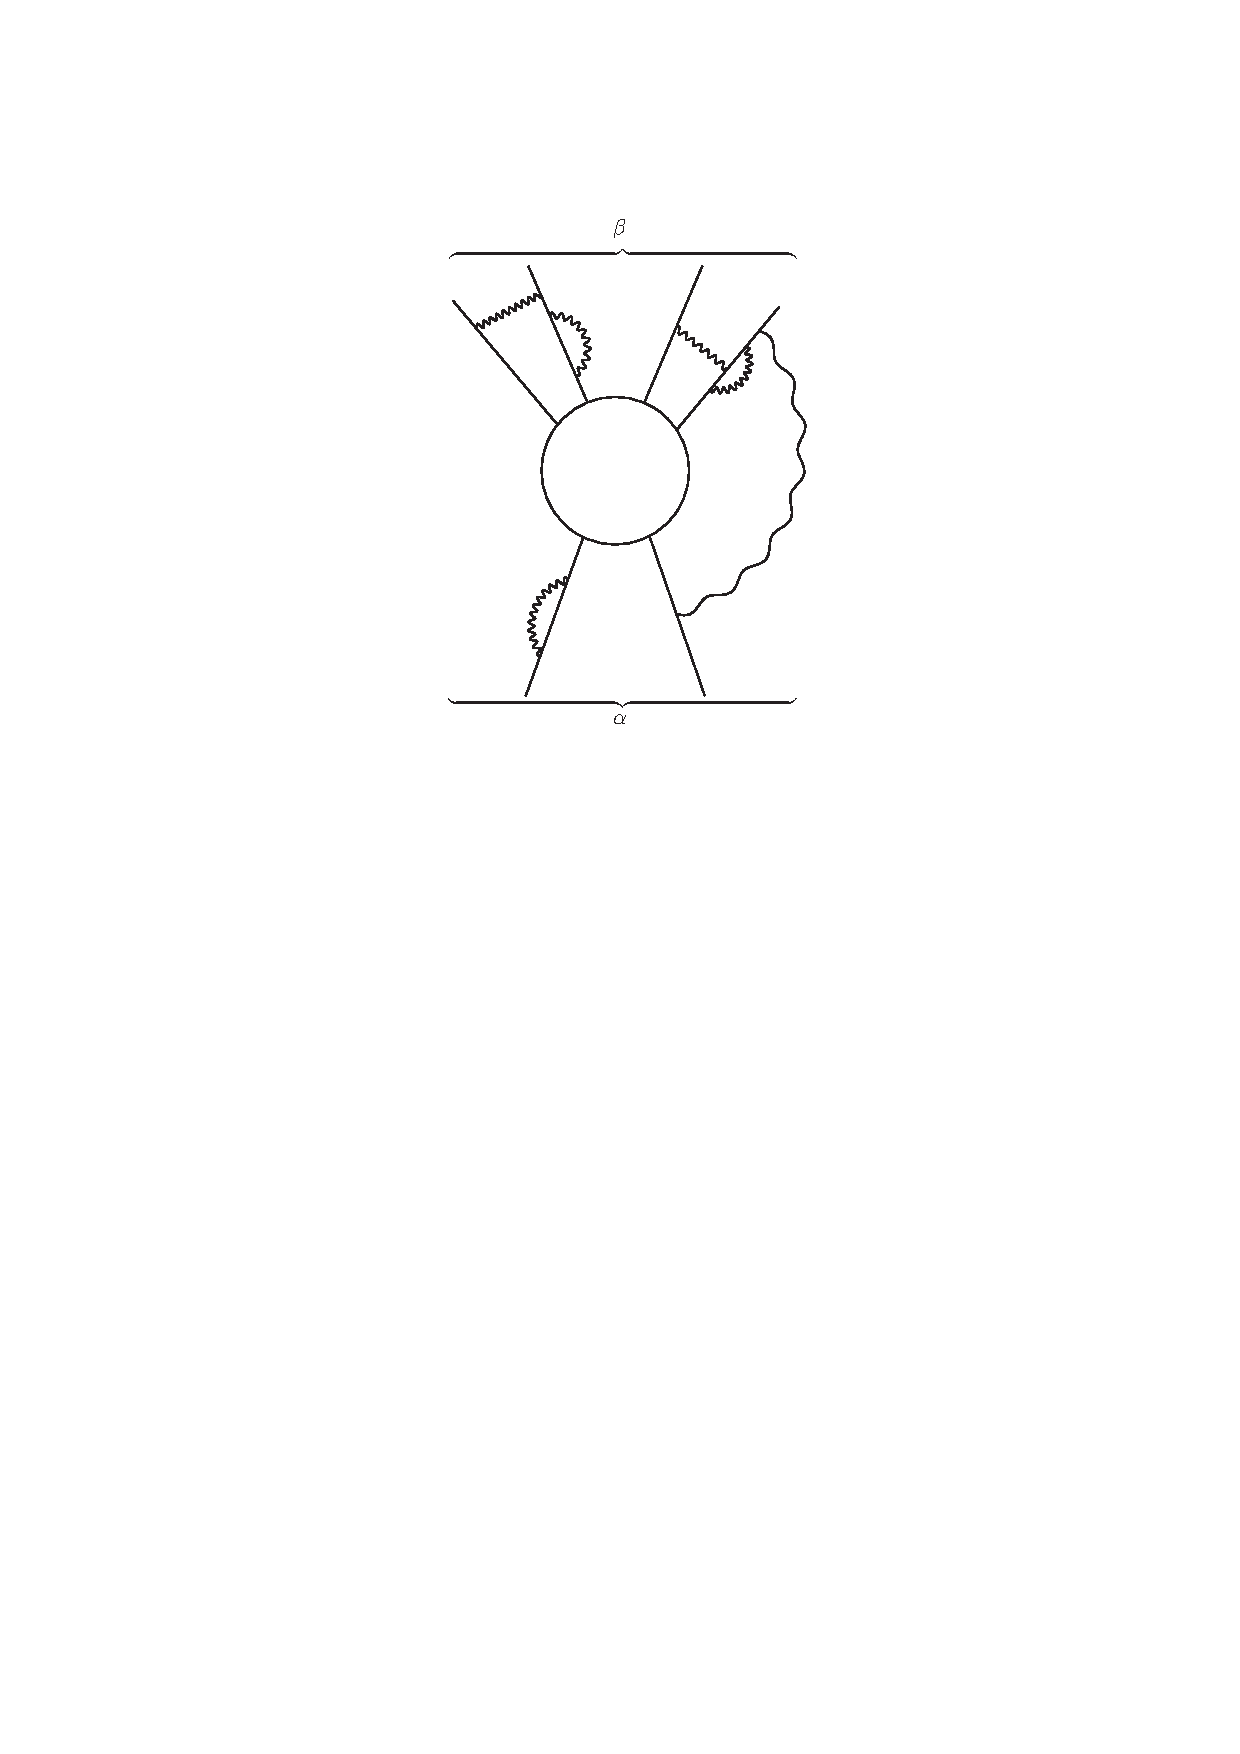
\includegraphics{figs/fig8.pdf}
	\caption{虚软光子辐射修正}
\end{figure}
把虚软光子看作是一个外腿辐射$q$的软光子,而另外一个外腿辐射$-q$的软光子,这样就可以利用前面的软定理的结论,发现最终的修正只是多了一个因子:
\begin{equation}
	J_{mn}\equiv\int_{\lambda<|\mathbf{q}|<\Lambda} \frac{d^4q}{(2\pi)^4}\frac{-i g_{\mu\nu}}{q^2-i0^+}\cdot\frac{\eta_mQ_m p^\mu_m}{p_m\cdot(-q)-i\eta_m 0^+}\cdot\frac{\eta_nQ_n p^\nu_n}{p_n\cdot(q)-i\eta_n 0^+} 
\end{equation}
这里光子的传播子选取了费曼规范。考虑$N$个虚光子的辐射修正,需要对$m,n$对于所有可能的外线进行求和,光子线置换和光子线两端求和会引入重复,所以还需要除以$N!2^N$因子:
\begin{equation}
	M_{\lambda}=M_\Lambda\cdot\frac{1}{N!2^N}\left(\sum_{n,m}J_{nm}\right)^N=M_{\Lambda}\exp\left[\frac{1}{2}\sum_{n,m}J_{nm}\right]
\end{equation}
将$J_{mn}$中的$\frac{Q_nQ_m\eta_n\eta_m}{(2\pi)^4}$抽离出来,剩下的积分部分记为$K_{mn}$,可以利用留数定理先计算$q^0$部分的积分:\begin{margintable}\footnotesize 
	\begin{tabularx}{\marginparwidth}{|X}
		极点为:
		\[\begin{aligned}q^0&=\frac{\mathbf{p}_m}{p_m^0}\cdot\mathrm{q}+\mathrm{i}\eta_m 0^+&q^0&=|\mathbf{q}|-\mathrm{i} 0^+\\q^0&=\frac{\mathbf{p}_n}{p_n^0}\cdot\mathrm{q}-\mathrm{i}\eta_n 0^+&q^0&=-|\mathbf{q}|+\mathrm{i} 0^+\end{aligned}\]
	\end{tabularx}
\end{margintable}
\begin{equation}
	K_{nm}=\begin{cases}
		-\pi(p_n\cdot p_m)\int_{\lambda\leq|\mathbf{q}|\leq\Lambda}\frac{\mathrm{d}^3q}{\left|\mathbf{q}\right|^3(E_n-\mathbf{\hat{q}}\cdot\mathbf{p}_n)(E_m-\mathbf{\hat{q}}\cdot\mathbf{p}_m)},&\eta_n=-\eta_m=\pm1\\
		-\pi(p_n\cdot p_m)\int_{\lambda\leq|\mathbf{q}|\leq\Lambda}\frac{\mathrm{d}^3q}{|\mathbf{q}|^3(E_n-\mathbf{\hat{q}}\cdot\mathbf{p}_n)(E_m-\mathbf{\hat{q}}\cdot\mathbf{p}_m)}-\frac{4\mathrm{i}\pi^3}{\beta_{nm}}\ln\left(\frac{\Lambda}{\lambda}\right),&\eta_n=\eta_m=\pm1
	\end{cases}
\end{equation}
其中
\[\beta_{nm}\equiv\sqrt{1-\frac{m_n^2m_m^2}{(p_n\cdot p_m)^2}}\]
这导致虚软光子修正的相因子对数发散,但我们最后实际可观测量是散射振幅的模方,所以最后这个虚数因子无关紧要,我们只需要关注$K_{nm}$的实部,可以统一的写为:
\begin{equation}
	\begin{aligned}
	\operatorname{Re}K_{mn}&=-\pi(p_n\cdot p_m)\int_{\lambda\leq|\mathbf{q}|\leq\Lambda}\frac{\mathrm{d}^3q}{|\mathbf{q}|^3(E_n-\mathbf{\hat{q}}\cdot\mathbf{p}_n)(E_m-\mathbf{\hat{q}}\cdot\mathbf{p}_m)}\\
	&=\frac{2\pi^2}{\beta_{nm}}\ln\biggl(\frac{1+\beta_{nm}}{1-\beta_{nm}}\biggr)\ln\biggl(\frac{\Lambda}{\lambda}\biggr)
	\end{aligned}
\end{equation}
\begin{remark}
	考虑非相对论量子力学中的散射问题时,需要求解径向波函数$R_\ell\equiv u_\ell$:
	\[-\frac{\hbar^2}{2m}\frac{d^2u}{dr^2}+\left[V(r)-\frac{\ell(\ell+1)\hbar}{2mr^2}\right]u_\ell=E_n u_\ell\]
	如果考虑$V(r)\propto\frac{1}{r}$的库伦散射,径向波函数的相因子并不是球面波的形式,也会出现对数发散:
	\[R_\ell(r)\sim\frac{\exp(\mathrm{i}pr-\mathrm{i}\nu\ln r)}{r}\]
	所以这里讨论的问题实际上时这个发散的相对论版本,非相对论版本的详尽分析见\cite{Schiff_1968}。
\end{remark}
将上式代入到振幅的模方表达式得到可观测量跃迁速率的修正:
\begin{equation}\label{23.5}
	\Gamma_{\lambda}=\left(\frac{\lambda}{\Lambda}\right)^{A}\Gamma_{\Lambda}
\end{equation}
其中:\sn{利用了$$\beta_{nm}=\begin{cases}
		0,&\eta_n\eta_m=+1\\
		\beta\in(0,1),&\eta_n\eta_m=-1
	\end{cases}$$}
\begin{equation}\label{23.6}
	A=-\frac{1}{8\pi^2}\sum_{nm}\frac{Q_nQ_m\eta_n\eta_m}{\beta_{nm}}\ln\left(\frac{1+\beta_{nm}}{1-\beta_{nm}}\right)=-\frac{Q^{2}}{8\pi^{2}}\left[4-\frac{2}{\beta}\ln\left(\frac{1+\beta}{1-\beta}\right)\right]
\end{equation}
$Q$是总电荷量。上式说明$A$总是大于0的,所以当$\lambda\to0$时,会导致$\Gamma_{\lambda}\to 0$,这意味着,考虑了虚软光子的修正之后,红外发散体现为QED中所有的过程都不可能发生!跃迁速率都是0!而这显然是不合常理的,这个发散会通过引入软光子辐射来消除,因为任意过程不但会在外腿之间传递任意数量的虚软光子,还会辐射出任意数量的,\textbf{不可探测的}实软光子。

根据前面的软定理,取模方并对螺旋度求和之后得到跃迁速率,然后再乘上相空间体积元,$\prod_{r=1}^N\frac{\mathrm{d}^3q_r}{(2\pi)^3(2|\mathbf{q}_r|)}$,得到辐射$N$个软光子到动量空间体积微元的微分速率:
\begin{equation}
	\mathrm d\Gamma_{\lambda}(\mathbf q_1,\cdots,\mathbf q_N)=\Gamma_{\lambda}\prod_{r=1}^{N}\frac{\mathrm d^3q_r}{(2\pi)^3(2|\mathbf q_r|)}\sum_{nm}\frac{\eta_n\eta_mQ_nQ_m(p_n\cdot p_m)}{(p_n\cdot q_r)(p_m\cdot q_r)}
\end{equation}

由于我们不可能分辨出能量无限低的软光子,所以我们测量到的跃迁速率应当是将那些所有可能的软光子发射位形积分之后得到的总的$\Gamma_{\lambda}(E,E_{T})$\sn{只要是我们看不到的过程,都要积分积掉!就像是在找边缘概率分布一样。},这里$E$,表示不可观测的软光子的能量都小于$E$,这里的$E_T$表示不管不可观测的软光子被辐射了多少,最终总的软光子能量都小于$E_T$。首先对软光子动量方向积分:
\begin{equation}
	\mathrm{d}\Gamma_{\lambda}(\omega_{1}\cdots\omega_{N})=\Gamma_{\lambda}A^{N}\frac{\mathrm{d}\omega_{1}}{\omega_{1}}\cdots\frac{\mathrm{d}\omega_{N}}{\omega_{N}}
\end{equation}
这里$A$就是\ref{23.6}。然后是对所有的软光子辐射数目可能求和,也就是对$N$求和,还要对软光子的能量积分,上限已经由$E,E_T$确定,下限同虚软光子一样是$\lambda$,最后将这个跑动参数定为$0$,后面将看到发散会抵消,理论不依赖于$\lambda$能标。
\begin{equation}
	\Gamma_{\lambda}(E,E_{T})=\Gamma_{\lambda}\sum_{N=0}^{\infty}\frac{A^{N}}{N!}\int_{E\geq\omega_{r}\geq\lambda,\sum_{r}\omega_{r}\leq E_{T}}\prod_{r=1}^{N}\frac{\mathrm{d}\omega_{r}}{\omega_{r}}
\end{equation}
引入阶跃函数:
\begin{equation}
	\theta(E_T-\sum_r\omega_r)=\frac{1}{\pi}\int_{-\infty}^{\infty}\mathrm{d}u\frac{\sin E_Tu}{u}\exp\left(\mathrm{i}u\sum_r\omega_r\right)
\end{equation}
可以将$\Gamma_{\lambda}(E,E_{T})$中积分简化为:
\begin{equation}
	\Gamma_{\lambda}(E,E_{T})=\frac{1}{\pi}\int_{-\infty}^{\infty}\mathrm{d}u\frac{\sin E_{T}u}{u}\exp\left(A\int_{\lambda}^{E}\frac{\mathrm{d}\omega}{\omega}\mathrm{e}^{\mathrm{i}\omega u}\right)\Gamma_{\lambda}
\end{equation}
指数中的积分可以通过写成$(\mathrm{e}^{\mathrm{i}\omega u}=1)/\omega$与$1/\omega$的积分之和,得到:
\begin{equation}
	\Gamma_{\lambda}(E,E_{T})\to\mathscr{F}\left(E/E_{T};A\right)\left(\frac{E}{\lambda}\right)^{A}\Gamma_{\lambda}
\end{equation}
其中:\sn{作了换元$u\to u/E_T,\omega\to E_T\omega$}
\begin{equation}
	\begin{aligned}
		\mathcal{F}(x;A)& \equiv\frac{1}{\pi}\int_{-\infty}^{\infty}\mathrm{d}u\frac{\sin u}{u}\exp\left(A\int_{0}^{x}\frac{\mathrm{d}\omega}{\omega}(\mathrm{e}^{\mathrm{i}\omega u}-1)\right)  \\
		&=1-\frac{A^{2}\theta(x-\frac{1}{2})}2\int_{1-x}^{x}\frac{\mathrm{d}\omega}\omega\ln\left(\frac{x}{1-\omega}\right)+\cdots 
	\end{aligned}
\end{equation}
如果$E/E_T\approxeq 1,A\ll 1$,则:
\begin{equation}
	\mathscr{F}\left(1;A\right)\simeq1-\frac{1}{12}\pi^2A^2+\cdots \to1
\end{equation}
然后注意到\ref{23.5},最终得到红外修正为:
\begin{equation}
	\Gamma_{\lambda}(E,E_{T})\to\mathscr{F}\left(E/E_{T};A\right)\left(\frac{E}{\Lambda}\right)^{A}\Gamma_{\Lambda}
\end{equation}
仅仅只是一个接近于1的因子,实际的计算上,我们使用费曼图计算$\Gamma_{\Lambda}$时圈积分在$\Lambda$以上做,而理论本身肯定是与这个“软”能标的选取无关的,所以实际计算上可以自由地选取$\Lambda$,使得$\mathscr{F}\to1,A\ll 1$,这样会使得前面的修正因子非常趋近于1,这样我们只需要计算来源于费曼图的$\Gamma_{\Lambda}$低阶贡献就能非常精确地得到$\Gamma_{\lambda}(E,E_{T})$的近似结果。

软引力子的红外发散抵消也可以类似的分析\cite{PhysRev.140.B516},非软粒子引起的一般的红外发散的处理参见\cite{Weinberg}$\S 13$。
\section{Massless QED}
本章用天球的视角来看QED理论,为下一节做准备,本节的讨论都局限于比较简单的,不含磁荷而且电子没有质量的QED理论,但是基于此推出的许多结论实际上是普适的,可以推广到有质量QED上\cite{Strominger:2017zoo}。
\subsection{Classical}
弯曲时空中QED作用量:
\begin{equation}
	S_{EM}=-\frac{1}{2e^2}\int{F}\wedge\star F +S_M=-\frac{1}{4e^2}\int \mathrm{d}^4x\sqrt{-g}F_{\mu]nu}F^{\mu\nu}+S_M
\end{equation}
其中$S_M$由$j^\nu A_\nu$形式给出相互作用项,即$j^\nu=-\frac{\delta S_M}{\delta A^\nu}$。Maxwell场方程有下面简洁形式:
\begin{equation}
	\begin{cases}
		dF=0&\Rightarrow \nabla_\mu F_{\nu\rho}+\nabla_\nu F_{\rho\mu}+\nabla_\rho F_{\mu\nu}=0\\
		d\star F=e^2\star j&\Rightarrow \nabla_\mu F_{\mu\nu}=e^2j_\nu
	\end{cases}
\end{equation}
下式给出了整个空间内的净电荷/磁荷\sn{后文$\star,*$指的都是Hodge dual}:
\begin{equation}
	Q_E=\frac{1}{e^2}\int_{\mathcal{S}^2_\infty}\star F=\int_{\Sigma}\star j,\quad Q_M=\frac{1}{2\pi}\int_{\mathcal{S}^2_\infty} F
\end{equation}
它们是量子化的,只能取整数。QED是$U(1)$规范理论,在$A\mapsto A+d\varepsilon$的规范变换下理论不变,后文不加说明都在所谓\textbf{retarded radial 规范}下进行计算\cite{He:2014cra,Kapec:2015ena}:
\begin{equation}
	\begin{aligned}
		&\mathcal{I}^+: A_r=0,\quad A_u|_{\mathcal{I}^+}=0\\
		&\mathcal{I}^-: A_r=0,\quad A_v|_{\mathcal{I}^-}=0
	\end{aligned}
\end{equation}
在$\mathcal{I}^{\pm}$附近可以把$A,F$展开成$\mathcal{O}(1/r)$的形式,用$A^{(i)},F^{(i)}$表示$r^{-i}$项前的系数,那么在这一规范下有\sn{各项系数都只和$(u,z,\bar z)$相关了}:
\begin{equation}
	F_{ur}^{(0)}=A_u^{(0)}, F_{z\bar z}^{(0)}=\partial_z A_{\bar z}^{(0)}-\partial_{\bar z}A_z^{(0)},F_{uz}^{(0)}=\partial_u A_z^{(0)},F_{rz}^{(0)}=-A_z^{(1)}
\end{equation}
而且我们所关心的场位形在$\mathcal{I}^{+}_{+}$处为真空,即满足:\sn{$\mathcal{I}^-_-$也是,就是前面说的C-K时空。}
\begin{equation}
	\left.F_{ur}\right|_{\mathcal{I}_{+}^{+}}=\left.F_{uz}\right|_{\mathcal{I}_{+}^{+}}=0
\end{equation}
$\mathcal{I}^-$处类似。但这个规范选取就如库伦规范$\nabla\cdot \mathbf{A}=0$一样没有完全确定规范,$A^{(0)}_z$还可以进行下面的所谓Large gauge transformation:
\begin{equation}
	A^{(0)}_z\mapsto A^{(0)}_z+\partial_z\varepsilon(z,\bar z),\quad \forall \varepsilon\in C^\infty\left[C\mathcal{S}^2\right]
\end{equation}
规范变换是一种冗余,但是这里的Large gauge transformations 最大的特点就是在无穷远处不归零,这导致很多时候分部积分的边界项不能丢去,确确实实的成为了一个对称性,后面马上会看到会对应无穷多个守恒荷。

运动电荷激发的电磁场即所谓Li\'enard\mbox{-}Wiecher势\cite{Jackson1998ClassicalE3}。这里我们在天球坐标下将advanced和retarded势统一写为:
\begin{equation}
	F_{rt}(\vec{x},t)=\frac{e^2}{4\pi}\sum_{k=1}^n\frac{Q_k\gamma_k\left(r-t\hat{x}\cdot\vec{\beta}_k\right)}{\left|\gamma_k^2\left(t-r\hat{x}\cdot\vec{\beta}_k\right)^2-t^2+r^2\right|^{3/2}},\quad r^2=\vec{x}\cdot\vec{x},\quad\vec{x}=r\hat{x}
\end{equation}
其中我们假设所有电荷之间匀速运动,而且相互作用可忽略,这个假设有点强,但是请\textbf{相信}后面导出的结论是可以推广到一般情形的。现在计算在天球上的极限:
\begin{equation}
	\begin{aligned}
		&\left.F_{rt}\right|_{\mathcal{I}^{+}}=\frac{e^{2}}{4\pi r^{2}}\sum_{k=1}^{n}\frac{Q_{k}}{\gamma_{k}^{2}(1-\hat{x}\cdot\vec{\beta}_{k})^{2}}\\
		&\left.F_{rt}\right|_{\mathcal{I}^{-}}=\frac{e^{2}}{4\pi r^{2}}\sum_{k=1}^{n}\frac{Q_{k}}{\gamma_{k}^{2}(1+\hat{x}\cdot\vec{\beta_{k}})^{2}}
	\end{aligned}
\end{equation}
取极限,得到:
\begin{equation}
	\boxed{
	\left.F_{rt}\right|_{\mathcal{I}^{+}_-}\neq \left.F_{rt}\right|_{\mathcal{I}^{-}_+}}
\end{equation}
正是这个式子说明了要严格区分$\mathcal{I}^{+}_-,\mathcal{I}^{-}_{+}$和$i^0$。但是,因为$F_{ru}=F_{rt}=F_{rv}$:
\begin{equation}
	\boxed{
		\lim\limits_{r\to\infty}r^2F_{ru}(\hat{x})\Big|_{\mathcal{I}_{-}^+}=\lim\limits_{r\to\infty}r^2F_{rv}(-\hat{x})\Big|_{\mathcal{I}_{+}^-}
	}
\end{equation}
也就是说场在两个天球上是对径认同的,这也是为什么前面$\mathcal{I}^{\pm}$天球的角向选取是antipodal的,上边的式子可以写成下面很简洁的形式:
\begin{equation}\label{24.12}
	\boxed{
	\left.F_{ru}^{(2)}(z,\bar z)\right|_{\mathcal{I}^{+}_-}=\left.F_{rv}^{(2)}(z,\bar z)\right|_{\mathcal{I}^{-}_+}
	}
\end{equation}
这个式子是普适的,而且非常重要,是后面散射问题的核心。上面的式子破缺了$\mathcal{I}^+\times\mathcal{I}^-$上的Large gauge,如$\mathrm{BMS}^+\times \mathrm{BMS}^-$一样破缺为一个diagonal的子群,现在考虑任意一个天球上的对径认同的函数:\sn{在$\mathcal{I}^\pm$上定义但是与$u,v$无关的函数,在$\mathcal{I}^\pm_\mp$上对径认同。}
\begin{equation}
	\varepsilon(z,\overline{z})|_{\mathcal{I}_{-}^{+}}=\varepsilon(z,\overline{z})|_{\mathcal{I}_{+}^{-}}
\end{equation}
定义下面的future charges和past charges:
\begin{equation}
	\boxed{
		Q_{\varepsilon}^{+}=\frac{1}{e^{2}}\int_{\mathcal I_{-}^{+}}\varepsilon*F,\quad Q_{\varepsilon}^{-}=\frac{1}{e^{2}}\int_{\mathcal I_{+}^{-}}\varepsilon*F
	}
\end{equation}
由于Hodge对偶后出来的体积元$\propto r^2$,所以在天球上$r\to\infty$,$F\to F^{(2)}$,再根据对径认同的条件,这样对于任意一个函数$\varepsilon$,我们都给出了一个“电荷”守恒律:
\begin{equation}
	\boxed{
	Q_\varepsilon^+=Q_\varepsilon^-
	}
\end{equation}
对于$\varepsilon$是常函数情形,就得到了一般的电荷守恒律。利用Stokes公式\sn{$\int_{\partial \Omega}\omega =\int_{ \Omega}d\omega$}可以改写$Q_\varepsilon^{\pm}$为\sn{$Q_\varepsilon^-$只用把$+\mapsto -$}:
\begin{equation}
	Q_\varepsilon^+=\frac{1}{e^2}\int_{\mathcal{I}^+}\mathrm{d}\varepsilon\wedge*F+\int_{\mathcal{I}^+}\varepsilon*j+\cancelto{0}{\frac{1}{e^2}\int_{\mathcal{I}_+^+}\varepsilon*F}
\end{equation}
最后一项为0是因为我们假设电子是无质量的,这样电子就是从$\mathcal{I}^-\to\mathcal{I}^+$,而不是$i^{-}\to i^+$,所以$F|_{\mathcal{I}_+^{+}}=0$。第一项是Soft term $Q_S^+$与软光子的产生湮灭有关,第二项由于是与流耦合,所以叫Hard term $Q_H^+$与带电实物粒子有关。将上面的微分形式写成分量形式\sn{其中使用了Bianchi恒等式:$\partial_{u}F_{ru}^{(2)}+D^{z}F_{uz}^{(0)}+D^{\bar{z}}F_{u\bar{z}}^{(0)}+e^2j_{u}^{(2)}=0$}:
\begin{equation}
	Q_{\varepsilon}^{+}=\underbrace{-\frac{1}{e^{2}}\int_{\mathcal{I}^{+}}dud^{2}z\left(\partial_{z}\varepsilon F_{u\bar{z}}^{(0)}+\partial_{\bar{z}}\varepsilon F_{uz}^{(0)}\right)}_{Q_{S}^{+}}+\underbrace{\int_{\mathcal{I}^{+}}dud^{2}z\varepsilon\gamma_{z\bar{z}}j_{u}^{(2)}}_{Q_{H}^{+}}
\end{equation}
定义Soft photon mode $N_z$:
\begin{equation}\label{eq:23.18}
	N_{z}\equiv \int_{-\infty}^{\infty}duF_{uz}^{(0)}=\lim_{\omega\to0}\int_{-\infty}^{\infty}duF_{uz}^{(0)}e^{i\omega u}
\end{equation}
再次看到$N_z$对应的是电磁场的零频部分,也就是软光子部分,而且有:
\begin{equation}
	\begin{aligned}
		\partial_{\bar{z}}N_{z}-\partial_{z}N_{\bar{z}}& =\int_{-\infty}^{\infty}du\left[\partial_{\bar{z}}F_{uz}^{(0)}-\partial_{z}F_{u\bar{z}}^{(0)}\right]  \\
		&=-\int_{-\infty}^{\infty}du\left.\partial_{u}F_{z\bar{z}}^{(0)}=-F_{z\bar{z}}^{(0)}\right|_{\mathcal{I}_{-}^{+}}^{\mathcal{I}_{+}^{+}}=0
	\end{aligned}
\end{equation}
最后等于0是因为$F_{z\bar z}|_{\mathcal{I}_{+}^{\pm}}=0$,本质上是因为没有磁单极子,磁场不是long-range的,在无穷远处为0\sn{因为$F_{z\bar z}=\frac{\partial x^{\mu}}{\partial z}\frac{\partial x^{\nu}}{\partial\bar{z}}F_{\mu\nu}=\frac{\partial x^{i}}{\partial z}\frac{\partial x^{j}}{\partial\bar{z}}F_{ij}$,而规范场强的空间分量$F_{ij}$只和磁场有关。}。所以$N_z$无旋,可以由此引申出一个实标量场$N$作为其原函数:
\begin{equation}
	N_z\equiv e^2\partial_zN=\int_{-\infty}^{\infty}duF_{uz}^{(0)}=A_{z}^{(0)}|_{\mathcal{I}_{+}^{+}}-A_{z}^{(0)}|_{\mathcal{I}_{-}^{+}}
\end{equation}
利用$N$,future charges可以写成下面简洁形式:
\begin{equation}\label{eq:23.21}
	Q_{\varepsilon}^{+}=2\int_{\mathcal{S}_\infty^2} d^{2}zN\partial_{z}\partial_{\bar{z}}\varepsilon+\int_{\mathcal I^{+}}dud^{2}z\varepsilon\gamma_{z\bar{z}}j_{u}^{(2)}
\end{equation}
对past charge也可以来上面的这一套:
\begin{equation}\label{eq:23.21.2}
	Q_{\varepsilon}^{-}=-2\int_{\mathcal{S}_\infty^2} d^{2}zN^-\partial_{z}\partial_{\bar{z}}\varepsilon+\int_{\mathcal I^{-}}dvd^{2}z\varepsilon\gamma_{z\bar{z}}j_{v}^{(2)}
\end{equation}
\begin{remark}
	正文里面省去了一些推导细节,在retarded下的Maxwell方程形式罗列如下:
	\begin{equation}
		\begin{aligned}(\partial_u-\partial_r)\left(r^2F_{ru}\right)+\gamma^{z\bar{z}}\left(\partial_zF_{u\bar{z}}+\partial_{\bar{z}}F_{u\bar{z}}\right)&=-e^2r^2j^M_u\\-\partial_r\left(r^2F_{ru}\right)+\gamma^{z\bar{z}}\left(\partial_zF_{r\bar{z}}+\partial_{\bar{z}}F_{r\bar{z}}\right)&=-e^2r^2j^M_r\\r^2\left(\partial_u-\partial_r\right)F_{r\bar{z}}+r^2\partial_rF_{u\bar{z}}+\partial_z\left(\gamma^{z\bar{z}}F_{z\bar{z}}\right)&=-e^2r^2j^M_z\end{aligned}
	\end{equation}
	Lorenz规范形式为:
	\begin{equation}
		-\partial_u\left(r^2A_r\right)-\partial_r\left(r^2A_u\right)+\partial_r\left(r^2A_r\right)+\gamma^{z\bar{z}}\left(\partial_zA_{\bar{z}}+\partial_{\bar{z}}A_z\right)=0
	\end{equation}
\end{remark}
\subsection{Quantization}
上面讨论的都是经典场,现在进行量子化,目的是说明前面定义的future charge 和 past charges 都是 Large gauge transformations 对应的生成元算符。量子化方案选用正则量子化方案,这里使用的方法不需要事先对时空进行3+1分解,是协变的方法\cite{Ashtekar1987AsymptoticQ,Frolov:1979ab,1989thyg.book.....H,Lee:1990nz,Wald:1999wa}。

经典力学的正则形式是建立在辛几何上的,也就是给相流形上配备了一个非退化的、闭的二形式\cite{Arnold}:
\begin{equation}\label{eq:23.22}
	\Omega=\frac{1}{2}\omega_{IJ}dx^I\wedge dx^J
\end{equation}
而且可以证明,可以通过选取不同的广义坐标局部的将$\omega_{IJ}$化为下面的矩阵:
\begin{equation}
	\omega_{IJ}=\left.\left[\begin{matrix}0&1_{N\times N}\\-1_{N\times N}&0\end{matrix}\right.\right]
\end{equation}
力学量的Possion括号由下式给定:
\begin{equation}
	\{A,B\}=\Omega^{IJ}\partial_IA\partial_JB
\end{equation}
相空间是运动方程的解,可以与初始值一一对应。

到了场论这边,相空间我们可以选取为某一个柯西面$\Sigma$上的场位形。场$\phi$本身是流形上的微分形式,\ref{eq:23.22}中的$dx$应该替换为$\delta\phi$,这里$\delta$是场位形的在壳变分,也就是说$\phi+\delta \phi$仍然是场方程的解。场本身是定义在某个纤维丛上的,可以粗浅的理解为两个流形拼起来,而$d$是底流形上的微分形式算子,$\delta$事实上是另一个正交的微分形式算子,所以$\delta\phi$在$\delta$的意义上是1\mbox{-}form,在$d$的意义上$\delta$的作用不会改变其是几形式,这样$\Omega$形如$\delta\phi\wedge\delta\varphi$从$\delta$的意义上看就是个二形式。构建的微分形式还应当满足规范不变性,闭且非退化,而且还要对柯西面的不同选取一致,利用\cite{Wald:1999wa}中方法可以得到$U(1)$规范场的辛形式为:
\begin{equation}
	\Omega_{\Sigma}=-\frac{1}{e^{2}}\int_{\Sigma}\delta(*F)\wedge\delta A
\end{equation}
将柯西面选取为$\mathcal{I}^{\pm}$,得到分量为:
\begin{equation}
	\begin{aligned}
		\omega_{uz\bar{z}}|_{\mathcal{I}}+& =-\frac{1}{e^{2}}\left[\delta(*F)_{uz}\wedge\delta A_{\bar{z}}+\delta(*F)_{\bar{z}u}\wedge\delta A_{z}+\delta(*F)_{z\bar{z}}\wedge\delta A_{u}\right]_{\mathcal{I}^{+}}  \\
		&=-\frac{i}{e^{2}}\left[\delta F_{uz}^{(0)}\wedge\delta A_{\bar{z}}^{(0)}+\delta F_{u\bar{z}}^{(0)}\wedge\delta A_{z}^{(0)}\right],
	\end{aligned}
\end{equation}
其中利用了:\sn{注意到Levi-Civita符号不是张量,而是张量密度,$\sqrt{-g}\epsilon$才是张量,然后利用Hodge dual定义爆算即可}
\begin{equation}
	(*F)_{uz}=i\left(F_{uz}-F_{rz}\right),\quad(*F)_{z\bar{z}}=ir^{2}\gamma_{z\bar{z}}F_{ru}
\end{equation}
最终得到辛形式:
\begin{equation}\label{eq:23.29}
	\Omega_{\mathcal{I}^+}=\frac{1}{e^2}\int dud^2z\left[\delta F_{uz}^{(0)}\wedge\delta A_{\bar{z}}^{(0)}+\delta F_{u\bar{z}}^{(0)}\wedge\delta A_{z}^{(0)}\right]
\end{equation}
总是可以把$A_z$的$u\to\pm {\infty}$,也就是$\mathcal{I}^+_{\pm}$的与$u$无关的部分分离出去,这一部分又总是可以写成某个天球上标量场的导数,因为要求$F_{z\bar z}|_{\mathcal{I}_{+}^{\pm}}=0$:\sn{这里所做的事情实际上是为了构建包含软光子模式$\{\phi,N\}$的协变相空间做准备,Strominger原始文献\cite{He:2014cra}(那里使用$\{\phi_\pm\}$代替这里的式$\{\phi,N\}$)就指出,如果不这样做会导致计算得出$Q^\pm_\varepsilon$不是Large规范变换的生成元}
\begin{equation}
	A_z^{(0)}(u,z,\bar{z})=\hat{A}_z(u,z,\bar{z})+\partial_z\phi(z,\bar{z}),\quad\partial_z\phi\equiv\frac{1}{2}\left[\left.A_z^{(0)}\right|_{\mathcal I_+^+}+\left.A_z^{(0)}\right|_{\mathcal I_-^+}\right]
\end{equation}
而且$\partial_z \phi$是一个pure gauge。利用上面的分解以及soft photon mode重写\ref{eq:23.29}:
\begin{equation}
	\Omega_{\mathcal{I}^{+}}=\frac{2}{e^{2}}\int dud^{2}z\partial_{u}\delta\hat{A}_{z}\wedge\delta\hat{A}_{\bar{z}}-2\int d^{2}z\partial_{z}\delta\phi\wedge\partial_{\bar{z}}\delta N
\end{equation}
现在考虑正则量子化,场变成算符,而Poisson括号换成Dirac括号:\sn{$\{\quad,\quad\}\mapsto\frac{1}{i}[\quad,\quad]$}
\begin{equation}
	\begin{aligned}-\frac{2}{e^2}\left[\partial_u\hat A_z(u,z,\bar z),\hat A_{\bar w}(u',w,\bar w)\right]&=i\delta(u-u')\delta^2(z-w),\\2\left[\partial_z\phi(z,\bar z),\partial_{\bar w}N(w,\bar w)\right]&=i\delta^2(z-w).\end{aligned}
\end{equation}
积分得到:\sn{这里$$\Theta(u)=\frac{1}{\pi i}\int\frac{d\omega}{\omega}e^{i\omega u}=\begin{cases}+1&,u>0\\-1&,u<0\end{cases}$$}
\begin{equation}
	\begin{aligned}
		\left[\hat{A}_{z}(u,z,\bar{z}),\hat{A}_{\bar{w}}(u^{\prime},w,\bar{w})\right]& =-\frac{ie^{2}}{4}\Theta(u-u^{\prime})\delta^{2}(z-w),  \\
		[\phi(z,\bar{z}),N(w,\bar{w})]& =-\frac{i}{4\pi}\log|z-w|^{2}+f(z,\bar{z})+g(w,\bar{w}). 
	\end{aligned}
\end{equation}

\subsection{Large guage symmetry}
利用上面发展的对易式可以去计算$Q_\varepsilon^{\pm}$与场算符的对易关系,注意到物质场部分$Q_H$始终和规范场$A$对易,所以:
\begin{equation}
	\begin{aligned}&\left[Q_{\varepsilon}^{+},A_{z}^{(0)}(u,z,\bar{z})\right]=i\partial_{z}\varepsilon(z,\bar{z}),\\&\left[Q_{\varepsilon}^{-},A_{z}^{(0)}(v,z,\bar{z})\right]=i\partial_{z}\varepsilon(z,\bar{z}).\end{aligned}
\end{equation}
所以前面定义的守恒荷其实就是对径认同的Large gauge transformation的生成元,自然就是一个守恒荷!下面是另外一些比较有用的对易关系:
\begin{equation}\label{eq:23.37}
	\left[Q_{\varepsilon}^{+},N(z,\bar{z})\right]=0,\quad\left[Q_{\varepsilon}^{+},\hat{A}_{z}(u,z,\bar{z})\right]=0,\quad\left[Q_{\varepsilon}^{+},\phi(z,\bar{z})\right]=i\varepsilon(z,\bar{z})
\end{equation}

前面的讨论一直忽略了流耦合项$S_M$,加入后对前面的结论不会有影响,注意到$Q_S$与物质场对易,根据Noether定理:
\begin{equation}
	\left[j_{u}^{(2)}(u',w,\bar{w}),\Phi_{k}(u,z,\bar{z})\right]=-Q_{k}\Phi_{k}(u,z,\bar{z})\gamma^{z\bar{z}}\delta^{2}(z-w)\delta(u-u')
\end{equation}
这意味着:
\begin{equation}\label{23.36}
	\left[Q_\varepsilon^+,\Phi_k(u,z,\bar{z})\right]=\left[\int_{\mathcal{I}^+}\varepsilon*j,\Phi_k(u,z,\bar{z})\right]=-Q_k\varepsilon(z,\bar{z})\Phi_k(u,z,\bar{z})\equiv i\delta_\varepsilon\Phi_k(u,z,\bar{z})
\end{equation}
所以$Q_S$生成规范场的规范变换,$Q_H$生成费米场规范变换,合起来$Q_\varepsilon$生成$\mathcal{I}^+$上的local规范变换。
\section{Ward indentity = Soft theorem}
\subsection{Ward indentity of $\mathcal{S}$\mbox{-}Matrix}
量子力学里面就知道守恒意味着与哈密顿量对易,而$\mathcal{S}\sim \exp{iHT}$,所以前面的守恒荷会和$\mathcal{S}$对易:\sn{初末态基底选取平面波。}
\begin{equation}\label{eq:24.1}
	\boxed{\langle\mathrm{out}|\left(Q_\varepsilon^+\mathcal{S}-\mathcal{S}Q_\varepsilon^-\right)|\mathrm{in}\rangle=0}
\end{equation}
这样一个简单的式子就是$\mathcal{S}$\mbox{-}Matrix的Ward identity。利用\ref{eq:23.21}和\ref{eq:23.21.2}得到:
\begin{equation}\label{eq:24.2}
	\begin{aligned}
		Q_\varepsilon^-|\mathrm{in}\rangle&=-2\int d^2z\partial_{\bar{z}}\varepsilon\partial_zN^-(z,\bar{z})|\mathrm{in}\rangle+\sum_{k=1}^mQ_k^\mathrm{in}\varepsilon(z_k^\mathrm{in},\bar{z}_k^\mathrm{in})|\mathrm{in}\rangle \\
		\langle\mathrm{out}|Q_\varepsilon^+&=2\int d^2z\partial_z\partial_{\bar{z}}\varepsilon\langle\mathrm{out}|N(z,\bar{z})+\sum_{k=1}^nQ_k^\mathrm{out}\varepsilon(z_k^\mathrm{out},\bar{z}_k^\mathrm{out})\langle\mathrm{out}|
	\end{aligned}
\end{equation}
第一项没啥好说的,后面会讨论其物理含义,第二项的计算稍微提一下。首先我们假设入射态是$m$个hard particles,而且来自于天球上的点$z_k^{\mathrm{in}}$,\ref{23.36}给出了守恒荷与物质场之间的对易关系,实际上,不难证明守恒荷和产生湮灭算符也满足同样的对易关系\sn{比如标量场\cite{srednicki}$$a^{\dagger}(\mathbf{k})=-i\int d^{3}xe^{ikx}\stackrel{\leftrightarrow}{\partial_{0}}\varphi(x)$$}。以两个入射粒子为例:
\begin{equation}
	\begin{aligned}
		Q^-_{H}\ket{\text{in}}&\sim Q^-_{H}a_1^\dagger a_2^\dagger\ket{0}\\
		&\sim \left[Q^-_{H},a_1^\dagger a_2^\dagger\right]\ket{0}+\cancelto{0}{a_1^\dagger a_2^\dagger Q^-_{H}\ket{0}}\\
		&\sim  \left[Q^-_{H},a_1^\dagger \right]a_2^\dagger\ket{0}+a_1^\dagger\left[Q^-_{\varepsilon},a_2^\dagger \right]\ket{0}\\
		&\sim Q_1\varepsilon_1\ket{\text{in}}+Q_2\varepsilon_2\ket{\text{in}}
	\end{aligned}
\end{equation}
第二行我们利用了真空态一定是没荷的\sn{后面对称性自发破缺会提到$Q^-_\varepsilon$作用到真空上不是0,但是这里$Q_H$是没有破缺的对称性。}。现在可以把\ref{eq:24.1}写为:
\begin{equation}\label{eq:25.4}
	\begin{aligned}
		2\int d^2z\partial_z\partial_{\bar{z}}\varepsilon\langle\text{out}|&\left(N(z,\bar{z})\mathcal{S}-\mathcal{S}N^-(z,\bar{z})\right)|\text{in}\rangle\\&=\left[\sum_{k=1}^mQ_k^\text{in}\varepsilon(z_k^\text{in},\bar{z}_k^\text{in})-\sum_{k=1}^nQ_k^\text{out}\varepsilon(z_k^\text{out},{\bar{z}}_k^\text{out})\right]\langle\text{out}|\mathcal{S}|\text{in}\rangle
	\end{aligned}
\end{equation}
取$\varepsilon(z,\bar z)=\frac{1}{w-z}$,则上式可以写为如下形式:\sn{$$\partial_{\bar{z}}\frac{1}{z-w}=2\pi\delta^2(z-w)$$最后$w\leftrightarrow z$}
\begin{equation}\label{eq:24.5}
	4\pi\langle\mathrm{out}|\left(\partial_zN\mathcal{S}-\mathcal{S}\partial_zN^-\right)|\mathrm{in}\rangle=\left[\sum_{k=1}^m\frac{Q_k^\mathrm{in}}{z-z_k^\mathrm{in}}-\sum_{k=1}^n\frac{Q_k^\mathrm{out}}{z-z_k^\mathrm{out}}\right]\langle\mathrm{out}|\mathcal{S}|\mathrm{in}\rangle 
\end{equation}
这个等式其实就是带有U(1) K$\breve{\text{a}}$c-Moody current的$\text{CFT}_2$的Ward恒等式\cite{Blumenhagen:2009zz,He:2015zea,Strominger:2013lka,Nande:2017dba},在介绍CFT后会专门讨论。这里的$\varepsilon$的选取是为了后面与正螺旋度光子的软定理联系,如果考虑负螺旋度的情况,可以选取$\varepsilon(z,\bar z)=\frac{1}{\bar w-\bar z}$进行一样的推导。这一$\varepsilon$的选取是有非常强的物理上的motivation的,因为后面推导的是单个软光子辐射的软定理,那自然想到只在天球上的某一个点上(这个点正代表着出射软光子$\hat p$)做large guage变换,所以$\delta A_z\sim\partial_z\varepsilon\sim\delta(\cdot)$,这正对应了我们此处的选取。

\subsection{Mode expansion}
本部分的终极目标是证明Ward恒等式可以联系渐近对称性和软定理,前文从相空间角度给出了Ward恒等式,在动量空间给出了软定理,是时候在动量空间重写Ward恒等式了,重点就是将场算符用平面波展开,也就是正则量子化的过程。free mode expansion 弯曲时空量子力学领域已经不少人算过了,U(1)规范理论结果如下:
\begin{equation}
	A_{\nu}(x)=e\sum_{\alpha=\pm}\int\frac{d^3q}{\left(2\pi\right)^3}\frac{1}{2\omega_q}\left[\varepsilon_{\nu}^{*\alpha}(\vec{q})a_{\alpha}^{\mathrm{out}}(\vec{q})e^{iq\cdot x}+\varepsilon_{\nu}^{\alpha}(\vec{q})a_{\alpha}^{\mathrm{out}}(\vec{q})^\dagger e^{-iq\cdot x}\right]
\end{equation}
$q$是平面波在壳动量$q^2=0$,$\varepsilon^\pm_\mu$是极化矢量,常常取为:
\begin{equation}\label{eq:24.7}
	\varepsilon^{+\mu}(\vec{q})=\frac1{\sqrt{2}}\left(\bar{z},1,-i,-\bar{z}\right),\quad\varepsilon^{-\mu}(\vec{q})=\frac1{\sqrt{2}}\left(z,1,i,-z\right),\quad q_{\mu}\varepsilon^{\pm\mu}(\vec{q})=0,\quad\varepsilon_{\alpha}^{\mu}\varepsilon_{\beta\mu}^{*}=\delta_{\alpha\beta}
\end{equation}
产生湮灭算符之间满足对易关系:
\begin{equation}
	\left[a_\alpha^{\mathrm{out}}(\vec q),a_\beta^{\mathrm{out}}(\vec q')^\dagger\right]=\delta_{\alpha\beta}(2\pi)^3(2\omega_q)\delta^3\left(\vec q-\vec q'\right)
\end{equation}
定义内积:
\begin{equation}
	(A,A')=-i\int d\Sigma^{\mu}[A^{\nu}(\nabla_{\mu}{A'}_{\nu}^{*}-\nabla_{\nu}{A'}_{\mu}^{*})-(A\leftrightarrow {A'}^{*})]
\end{equation}
这样定义的内积与类空超曲面$\Sigma$的选取是无关的。这样一来产生湮灭算符可以写成:
\begin{equation}
	a_\pm(q)=i({A},(\epsilon^\pm e^{iq\cdot x})^*)
\end{equation}
对于$\mathcal{I}^-$类似讨论,结果只是把out改成in。下面计算$A_z^{(0)}(u,z,\bar{z})\equiv\lim_{r\to\infty}A_z(u,r,z,\bar{z})$的模式展开:\sn{这里$\hat q,\hat x$都是指其空间部分}
\begin{equation}
	\begin{aligned}
		A_{\mu}(x) =&e\sum_{\alpha=\pm}\int\frac{d^3q}{\left(2\pi\right)^3}\frac{1}{2\omega_q}\left[\varepsilon_{\mu}^{*\alpha}(\vec{q})a_{\alpha}(\vec{q})e^{-i\omega_qu-i\omega_qr(1-\hat{q}\cdot\hat{x})}\right. \\
		&\left.+\varepsilon_{\mu}^{\alpha}(\vec{q})a_{\alpha}^{\dagger}(\vec{q})e^{i\omega_{q}u+i\omega_{q}r(1-\hat{q}\cdot\hat{x})} \right]\\
		=&\frac e{8\pi^2}\sum_{\alpha=\pm}\int_0^\infty d\omega_q\omega_q\int_0^\pi d\theta\sin\theta\left[\varepsilon_\mu^{*\alpha}(\vec{q})a_\alpha(\vec{q})e^{-i\omega_qu-i\omega_qr(1-\cos\theta)}\right. \\
		&\left.+\varepsilon_{\mu}^{\alpha}(\vec{q})a_{\alpha}^{\dagger}(\vec{q})e^{i\omega_{q}u+i\omega_{q}r(1-\cos\theta)}\right].
	\end{aligned}
\end{equation}
这里$\theta$是$\hat q$和$\hat x$之间的夹角,利用数学公式\sn{来源是鞍点近似}:
\begin{equation}
	\lim_{r\to\infty}\sin\theta e^{i\omega_qr(1-\cos\theta)}=\frac{i}{\omega_qr}\delta(\theta)+\mathcal{O}((r)^{-2})
\end{equation}
代入得到:
\begin{equation}
	A_\mu(x)=-\frac{ie}{8\pi^{2}r}\sum_{\alpha=\pm}\int_{0}^{\infty}d\omega_{q}\left[\varepsilon_{\mu}^{*\alpha}(\omega_{q}\hat{x})a_{\alpha}(\omega_{q}\hat{x})e^{-i\omega_{q}u}-c.c.\right]+\mathcal{O}(r^{-2})
\end{equation}
我们要求的玩意儿是$A_{z}=\partial_{z}x^{\mu}A_{\mu}$,注意到:
\[
	\partial_{z}x^{\mu}\varepsilon_{\mu}^{+}(\omega_{q}\hat{x})=0,\quad\partial_{z}x^{\mu}\varepsilon_{\mu}^{-}(\omega_{q}\hat{x})=\frac{\sqrt{2}r}{1+z\bar{z}}
\]
最终求得:\sn{下文中的$\omega$指$\omega_q$,即$q^0$}
\begin{equation}
	A_{z}^{(0)}(u,z,\bar{z})=-\frac{i}{8\pi^2}\frac{\sqrt{2}e}{1+z\bar{z}}\int_{0}^{\infty}d\omega\left[a_{+}^{\mathrm{out}}(\omega\hat{x})e^{-i\omega u}-a_{-}^{\mathrm{out}}(\omega\hat{x})^\dagger e^{i\omega u}\right]
\end{equation}
把定义式\ref{eq:23.18}改写为厄米的形式:
\begin{equation}
	\partial_zN=\dfrac{1}{2e^2}\lim_{\omega\to0^+}\int_{-\infty}^{\infty}du\left(e^{i\omega u}+e^{-i\omega u}\right)F_{uz}^{(0)}
\end{equation}
利用$A_z^{(0)}$重写上式为:
\begin{equation}
	\partial_zN=-\frac{1}{8\pi e}\frac{\sqrt{2}}{1+z\bar{z}}\lim_{\omega\to0^+}\left[\omega a_+^{\mathrm{out}}(\omega\hat{x})+\omega a_-^{\mathrm{out}}(\omega\hat{x})^\dagger\right]
\end{equation}
在$\mathcal{I}^-$上也有类似式子,只需要把$N\to N^-$,out$\to$in 就好。现在可以看出来为啥要叫soft photon mode 了。根据前面的铺垫,\ref{eq:24.5}终于可以写成如下形式:
\begin{equation}
	\begin{aligned}
		\operatorname*{lim}_{\omega\rightarrow0}\left\lfloor\omega\langle\mathrm{out}|\left(a_{+}^{\mathrm{out}}(\omega\hat{x})\mathcal{S}\right.\right.& \left.-\mathcal{S}a_{-}^{\mathrm{in}}(\omega\hat{x})^{\dagger}\right)|\mathrm{in}\rangle   \\
		&=\sqrt{2}e(1+z\bar{z})\left[\sum_{k=1}^{n}\frac{Q_{k}^\mathrm{out}}{z-z_{k}^\mathrm{out}}-\sum_{k=1}^{m}\frac{Q_{k}^\mathrm{in}}{z-z_{k}^\mathrm{in}}\right]\langle\mathrm{out}|\mathcal{S}|\mathrm{in}\rangle 
	\end{aligned}
\end{equation}
\subsection{Soft photon \& graviton}
前面用费曼图导出的软定理可以用$\mathcal{S}$矩阵写成如下形式:
\begin{equation}
	\lim\limits_{\omega\to0}\left[\omega\langle\text{out}|a_+^\text{out}(\vec{q})\mathcal{S}|\text{in}\rangle\right]=e\lim\limits_{\omega\to0}\left[\sum\limits_{k=1}^m\frac{\omega Q_k^\text{out}p_k^\text{out}\cdot\varepsilon^+}{p_k^\text{out}\cdot q}-\sum\limits_{k=1}^n\frac{\omega Q_k^\text{in}p_k^\text{in}\cdot\varepsilon^+}{p_k^\text{in}\cdot q}\right]\langle\text{out}|\mathcal{S}|\text{in}\rangle 
\end{equation}
这里出射和入射态都是平面波为基,而且我们把元电荷作为公因子提出,$Q\in\mathbb{Z}$,出入射动量用Embedding的形式写出来,前面第三部分写过,这里再写一遍:
\begin{equation}
	\begin{aligned}
		&q^{\mu} =\frac\omega{1+z\bar{z}}\left(1+z\bar{z},z+\bar{z},-i(z-\bar{z}),1-z\bar{z}\right),  \\
		&p_{k}^{\mu} =\frac{E_{k}}{1+z_{k}\bar{z}_{k}}\left(1+z_{k}\bar{z}_{k},z_{k}+\bar{z}_{k},-i(z_{k}-\bar{z}_{k}),1-z_{k}\bar{z}_{k}\right) 
	\end{aligned}
\end{equation}
注意到:
\begin{equation}
	\varepsilon_{+}^{\mu}(q)=\frac{1}{\sqrt{2}\omega}\partial_{z}\left[\left(1+z\bar{z}\right)q^{\mu}\right],\quad\varepsilon_{-}^{\mu}(q)=\frac{1}{\sqrt{2}\omega}\partial_{\bar{z}}\left[\left(1+z\bar{z}\right)q^{\mu}\right]
\end{equation}
带进去一通暴力计算,软定理被我们写成了:
\begin{equation}
\lim_{\omega\to0^+}\left[\omega\left\langle\mathrm{out}\right|a_+^\mathrm{out}(\omega\hat{x})\mathcal{S}\left|\mathrm{in}\right\rangle\right]\\=\frac{e}{\sqrt{2}}\left(1+z\bar{z}\right)\left[\sum_{k\in\mathrm{out}}\frac{Q_k}{z-z_k}-\sum_{k\in\mathrm{in}}\frac{Q_k}{z-z_k}\right]\left\langle\mathrm{out}\right|\mathcal{S}\left|\mathrm{in}\right\rangle
\end{equation}
根据${\mathcal{CPT}}$不变性:\sn{这里没搞懂为啥?}
\begin{equation}
\langle\text{out}|a_+^\text{out}(\vec{q})\mathcal{S}|\text{in}\rangle=-\langle\mathrm{out}|\mathcal{S}a_{-}^{\mathrm{in}\dagger}(\vec{q})|\mathrm{in}\rangle
\end{equation}
结合上面两个式子就证明了Ward恒等式和软定理是一回事,或者说通过Ward恒等式,软定理和 Large gauge symmetry 是一回事。这其实反过来说明了我们找到的 Large gauge symmetry 是non-trivial的,确实得看作是一个渐近对称性。这种non-trivial从记忆效应也能体现出来,后面会详细讨论。

回到引力这边,这边的证明思路上差不多,但是有很多比较微妙的点。首先就是守恒荷的量子化,虽然也可以按照QED那边的方法一样做,但是技术细节上微妙许多。不过我们可以猜测它们应当有如下形式:
\begin{equation}
	\boxed{
		\left[Q_f^+,\cdots\right]=i\delta_f,\quad \left[Q_Y^+,\cdots\right]=i\delta_Y
	}
\end{equation}
至于$\delta_f$和$\delta_Y$的形式前面已经算过了,而且它们都是和哈密顿量对易的,这也是利用Ward恒等式的基础。第一个式子证明相对简单,可以看文献\cite{He:2014laa},第二个等式要复杂许多,首先是需要下面几个式子\cite{Ashtekar1987AsymptoticQ,Ashtekar:1978zz,Ashtekar:1981bq,PhysRevLett.46.573}:
\begin{equation}
	\begin{aligned}
		\begin{bmatrix}N_{\bar{z}\bar{z}}(u,z,\bar{z}),C_{ww}(u',w,\bar{w})\end{bmatrix}&=16\pi Gi\gamma_{z\bar{z}}\delta^2(z-w)\delta(u-u')\\
		\left[Q_{S}^{+},C_{zz}\right]&=-iuD_{z}^{3}Y^{z},\\\left[Q_{H}^{+},C_{zz}\right]&=\frac{iu}{2}D\cdot YN_{zz}+iY\cdot DC_{zz}-\frac{i}{2}D\cdot YC_{zz}+2iD_{z}Y^{z}C_{zz}
	\end{aligned}
\end{equation}
而且Superrotation对应的相空间也更加复杂\cite{Strominger:2016wns}。这些都只能先argue一下,细说太麻烦。同样也可以给出模式展开,这个时候$g^{\mu\nu}=\eta^{\mu\nu}+\kappa h^{\mu\nu}$,$h^{\mu\nu}$满足linearized Einstein equation:
\begin{equation}
	\partial_{\sigma}\partial_{\nu}h^{\sigma}{}_{\mu}+\partial_{\sigma}\partial_{\mu}h^{\sigma}{}_{\nu}-\partial_{\mu}\partial_{\nu}h-\Box h_{\mu\nu}=0
\end{equation}
Mode expansion为:
\begin{equation}
	{h}_{\mu\nu}(x)=\kappa\sum_{\alpha\in\pm}\int\frac{d^3k}{(2\pi)^3}\frac{1}{2k^0}\left[\epsilon_{\mu\nu}^{\alpha*}a_{\alpha}e^{ik\cdot x}+\epsilon_{\mu\nu}^{\alpha}a_{\alpha}^{\dagger}e^{-ik\cdot x}\right]
\end{equation}
若$h=0$,内积定义为:
\begin{equation}
	(h,h')=-i\int d\Sigma^\rho[h^{\mu\nu}(\nabla_\rho {h'}_{\mu\nu}^*-2\nabla_\mu {h'}_{\rho\nu}^*)-(h\leftrightarrow {h'}^*)]
\end{equation}
同样也可以用鞍点近似去求度规里的那些参数的模式展开,然后去证明软引力子定理,详细的计算移步至文献\cite{Kapec:2014opa,He:2014laa,Campiglia:2014yka}。文献中详细论证了Supertranslation对应的守恒荷可以导出软定理的leading order,而$Q_Y$对应sub-leading order,计算过程十分复杂,后面对于比较简单的无质量标量QED的情况我们会细走一下这个过程。软引力子定理的sub-subleading order也被计算过了\cite{Cachazo:2014fwa},这也意味着有更高阶的守恒荷,文献\cite{Campiglia:2016efb}对此进行了分析。

\subsection{Asymptotic analysis on QED}
这一节的主要目的是讲一下历史进程,文献最早是通过类似于BMS的渐近分析得到守恒荷这些\cite{Strominger:2013lka,He:2014cra}。分析渐近对称性的第一步就是指定边界条件,从而找到允许的对称性。由于$T_{uu}$是能动张量$T_{00}$和$T_{0i}$的线性组合,所以它现在代表能流,由于天球半径按照$r^2$增大,所以为了让能量有限大,$T_{uu}\sim\mathcal{O}\left(\frac{1}{r^2}\right)$,根据Noether定理:
\begin{equation}
	T^{\mu\nu}=\frac{1}{16\pi}F^{\alpha\beta}F_{\alpha\beta}\eta^{\mu\nu}-\frac{1}{4\pi}F^{\mu\rho}\partial^{\nu}A_{\rho}
\end{equation}
进行对称化操作得到:\sn{这样子做最大的好处是现在不显含$A$,与规范无关了}
\begin{equation}
	T_{S}^{\mu\nu}\equiv T^{\mu\nu}-\frac{1}{4\pi}\partial_{\rho}\left(F^{\rho\mu}A^{\nu}\right)=\frac{1}{16\pi}F^{\alpha\beta}F_{\alpha\beta}\eta^{\mu\nu}-\frac{1}{4\pi}F^{\mu\rho}{F^{\nu}}_{\rho}
\end{equation}
改到Bondi坐标下:
\begin{equation}
	T_{uu}\sim F_{uz}F_{u\bar{z}}\frac{\gamma^{z\bar{z}}}{r^2}+\ldots 
\end{equation}
这个式子意味着$F_{uz}\sim\mathcal{O}(1)$,再根据$F_{ru},F_{rz}$是电磁场分量,所以渐近行为均为$\mathcal{O}(1/r^2)$。下面的一组$A$的渐近行为选取就满足这几个条件:\sn{这一节我们并不取定规范}\sn{这个条件充分但不必要,但是根据文献\cite{Campiglia:2016hvg,Conde:2016csj,Conde:2016rom}的讨论,选别的理论会变得不是很自然。}
\begin{equation}
	A_z\sim\mathcal{O}(1),\quad A_r\sim\mathcal{O}\left(\frac{1}{r^2}\right),\quad A_u\sim\mathcal{O}\left(\frac{1}{r}\right)
\end{equation}
而满足这一边界条件的规范变换只能是:
\begin{equation}\label{eq:24.32}
	\varepsilon=\varepsilon(z,\bar{z})+\mathcal{O}\left(\frac1r\right)
\end{equation}
无穷远(天球)处不归零,就是前面说的Large gauge transformations。类似于引力散射问题的分析,可以证明$\{A^0_z\}$是initial data,也就是说在$\mathcal{I}^+(\mathcal{I}^-)$上知晓了它就能将其它所有场在$\mathcal{I}^+(\mathcal{I}^-)$柯西面上的位形确定到只差一个积分常数。所以QED这边散射问题($\mathcal{I}^-\to\mathcal{I}^+$场位形的map问题)为了well-define,也必须把$\{A^0_z\}$对径认同的要求\begin{margintable}\footnotesize 
	\begin{tabularx}{\marginparwidth}{|X}
		$$\left.A^0_z\right|_{\mathcal{I}^+_-}=\left.A^0_z\right|_{\mathcal{I}^-_+}$$
	\end{tabularx}
\end{margintable}看作是散射问题定义的一部分。这样的话自然也就要求$\mathcal{I}^\pm$上的规范变换\ref{eq:24.32}互相对径认同。

历史上的发展和本文讨论的路线是完全相反的,2014年那段时间Strominger那些人首先是对QED和微扰引力直接去分析渐近对称性,然后去用Noether定理那一套去构建相应的守恒荷,再使用协变相空间方法进行量子化。过程中根据Lorentz不变性和$\mathcal{CPT}$的要求发现渐近对称性必须是对径认同变换的子群。而现在是把场在$\mathcal{I}^\pm_\mp$上对径认同放在第一性原理上面(看作是散射问题良定义的自然要求),然后引入天球上对径认同的函数去直接构造守恒荷,然后利用协变相空间进行量子化后发现这些守恒荷正是Large gauge/diffeomorphic 变换的生成元!

\section{Spontaneous symmetry breaking}
A. Zee\cite{Zee:2010qce}这部分物理讲的很清楚。
\subsection{In QFT}
考虑$\vec{\varphi}\equiv(\varphi_1,\varphi_2,\cdots,\varphi_N)$所定义的拉式量:
\begin{equation}
	\mathcal{L}=-\frac{1}{2}\left[(\partial\vec{\varphi})^2+\mu^2\vec{\varphi}^2\right]-\frac{\lambda}{4}(\vec{\varphi}^2)^2
\end{equation}
这个理论具有明显的$O(n)$对称性,但是我们可以“人为地”在理论中添加$\varphi_1^2,\varphi_1^3$等项来使得理论本身的对称性破坏为子群。还有一种是下面的模型,把质量项改成负的:
\begin{equation}
	\mathcal{L}=-\frac{1}{2}\left[(\partial\vec{\varphi})^2-\mu^2\vec{\varphi}^2\right]-\frac{\lambda}{4}(\vec{\varphi}^2)^2
\end{equation}
并不能解释为粒子具有“虚数”质量,而只能将质量项看作势能项的一部分。为了方便起见,考虑$N=2$的情形,势能项为:
\begin{equation}
	V(\vec{x})=-\frac{1}{2}{\vec{\varphi}}^2+\frac{\lambda}{4}(\vec{\varphi}^2)^2+\cancelto{0}{\frac{1}{2}(\nabla\varphi)^2}
\end{equation}
最后一项为0是因为正定,所以我们后面找真空态场位形要求能量最低可以干脆在那些不随空间变化的场位形里面找。势能的图像就是右边的典中典Mexican帽
\begin{marginfigure}
	\begin{center}
\begin{tikzpicture}[font=\footnotesize]
	\begin{axis}[
		axis lines=center,
		axis equal,
		domain=0:360,
		y domain=0:1.25,
		y axis line style=stealth-,
		y label style={at={(0.35,0.18)}},
		xmax=1.6,zmax=1.3,
		xlabel = $\varphi_{1}$,
		ylabel=$\varphi_{2}$,
		zlabel=$V(\vec{x})$,
		ticks=none
		]
		\addplot3 [surf,shader=flat,draw=black,fill=white,z buffer=sort] ({sin(x)*y}, {cos(x)*y}, {(y^2-1)^2});
		\coordinate (center) at (axis cs:0,0,1);
		\coordinate (minimum) at (axis cs:{cos(30)},{sin(30)},0);
	\end{axis}
	
	\fill[Blue] (center) circle (0.1);
	\fill[Red] (minimum) circle (0.1);
	\draw (center) edge[shorten <=5,shorten >=5,out=-10,in=150,double,draw=gray,double distance=0.5,-{>[length=2,line width=0.5]}] (minimum);
\end{tikzpicture}
\end{center}
\caption{对称性自发破缺}
\end{marginfigure}

这种势能会导致极(小)值点不唯一,也就是说真空态是简并的,而我们做量子场论都是要选定一个真空态之后在其附近微扰找激发态。真空态选择不影响物理,但是一旦你选定了一个真空态,就意味着体系原先有的$O(2)$对称性完全破缺了。所以说拉式量本身是对称的,但是真实世界由于选定了某个特殊的真空态,自发的破缺了对称性,导致我们现实中其实看不到体系的$O(2)$对称性。

不妨取定真空态为$\vec{\varphi}=(\sqrt{\mu^2/\lambda},0)$,然后在真空态附近展开场位形,即重定义场为:
\begin{equation}
	\varphi_1^\prime=\varphi_1-v+\mathcal{O}(\varphi^2),\quad \varphi_2^\prime=\varphi_2-0+\mathcal{O}(\varphi^2)
\end{equation}
代入原本的拉式量得到对称性自发破缺后的拉式量形式:\sn{最后把$\varphi^\prime$替换为$\varphi$}
\begin{equation}
	\mathcal{L}=\frac{\mu^4}{4\lambda}+\frac{1}{2}\left[(\partial\varphi_1)^2+(\partial\varphi_2)^2\right]-\mu^2\varphi_1^2+O(\varphi^3)
\end{equation}
对称性自发破缺带来了两个非常重要的东西:
\begin{itemize}
	\item \textbf{质量项}:现在$\varphi_1$的质量项是正定的,可以解释为质量
	\item \textbf{无质量玻色子}:多了一项$\varphi_2$,但是他是没有质量项的,我们称之为Nambu-Goldstone玻色子
\end{itemize}
$O(2)$对称性破缺有两个,一个是Abel的Lie群$SO(2)$的破缺,也就是说沿着帽中轴线的旋转对称性由于选取了一个特定的真空被破缺了,正是这种连续对称性的破缺,会有守恒荷的破缺,所以最终导致Nambu-Goldstone玻色子的产生。而$\mathbb{Z}_2$的离散对称性破缺不会带来无质量玻色子。
\begin{theorem}[Nambu-Goldstone]
	每一个连续对称性的破缺都会带来一个无质量Boson,称为Nambu-Goldstone Boson。
\end{theorem}
\begin{proof}
	从对称性没有自发破缺的拉式量中可以得出一些守恒荷,有一些是将要破缺的对称性对应的$Q_b$,也有一些是物理世界真实会看到的$Q$\footnote{Noether定理对连续对称性才有效,所以定理中才要强调连续对称性的破缺}。真空态自然是要求在物理真实世界的$Q$作用为0:\footnote{真空零点能可以通过重定义$H$消去}
	\begin{equation}
		H\ket{0}=Q\ket{0}=0
	\end{equation}
	但是对于破缺的对称性会有$Q_b\ket{0}\neq0$,但是根据$[H,Q_b]=0$可以说明$Q_b\ket{0}$还是一个真空态,所以破缺对称性对应的守恒荷作用在真空态上会把他变成另一个真空态。假设$D$为时空空间部分的维数,那么对于每一个守恒荷$Q_b=\int d^DxJ^0(\vec{x},t)$可以定义粒子态:
	\begin{equation}
		|s\rangle=\int d^{D}xe^{-i\vec{k}\vec{x}}J^{0}(\vec{x},t)|0\rangle 
	\end{equation}
	下面的推演说明了其是动量为$\vec{k}$的单粒子态:
	\begin{equation}
		P^{i}\left|s\right\rangle=\int d^{D}xe^{-i\vec{k}\vec{x}}[P^{i},J^{0}(\vec{x},t)]|0\rangle=-i\int d^{D}e^{-i\vec{k}\cdot\vec{x}}\partial^{i}J^{0}(\vec{x},t)|0\rangle=k^{i}|s\rangle 
	\end{equation}
	而且$Q_b\ket{0}=\lim\limits_{\vec{k}\to0}\ket{s}$,而这意味着$\vec{k}\to0$,$\ket{s}$能量也趋近于0,这意味着$\ket{s}$对应一个无质量粒子!这样我们就证明了定理。而$Q_b$对应的Goldstone玻色子到底是$\mathcal{L}$里面的哪个场可以通过计算$Q_b$与无质量场之间的对易子完成,因为无质量玻色子从物理上看就是因为破缺的对称性会让它沿着等势面无需能量进行移动,如果对易子不是0就说明$Q_b$恰恰生成的是这个Goldstone玻色子。
\end{proof}
但是上面的推导没有考虑量子真空涨落,在$D=2$时会失效:
\begin{theorem}[Coleman-Mermin-Wagner]
	空间维数为2的系统不可能发生连续对称性的破缺。
\end{theorem}
这里面还有一个微妙的地方,对于$D>2$的体系,真空态之间其实会有所谓的“超选择性”,也就是说前面虽然说$Q_b$可以把简并的真空态联系起来,但这个算符其实是不可归一化的,或者说对应无穷大的能量。
\subsection{On Celestial}
现在把天球上Large gauge symmetry的对称性自发破缺按照前面的框架进行讨论,但天球上的又存在许多subtle的地方。

对于QED,天球上的large规范变换实际上是在选取不同的真空,每一个$\varepsilon(z,\bar z)$就会对应一个真空,所以QED的真空是简并的,而且标记不同真空是用一个(对径认同)函数而不是一个连续参数,所以真空还是无穷维简并的,每一个$\varepsilon(z,\bar z)$便会带来一个对称性破缺的守恒荷$Q^+_\varepsilon$,从\ref{eq:23.37}可以看到$\left[Q_{\varepsilon}^{+},\phi(z,\bar{z})\right]\neq 0$,所以Large gauge symmetry破缺导致的Goldstone粒子是$\phi$对应的软光子!天球上的对称性自发破缺与一般的破缺最大的区别就是破缺对称性对应的守恒荷是normalizable的,不存在真空的超选择性,毕竟每个散射过程原则上都有无穷多的软光子产生湮灭。这个可以理解为天球上的简并真空是用一个local的函数标记的,而不是一般对称性破缺的一个global的连续参数,所以一般的对称性如果改变真空就需要牵一发而动全身,但是天球上真空的变化只需要合适的调整local函数,仅改变天球上的某一点,自然能量就有限大了。

不同真空态都是pure gauge,对应$F=0$,所以他们的$\left.Q^+_\varepsilon\right|_{\mathrm{vacuum}}$实际上都是0,所以说QED比较平庸。但是引力就不一样了,前面$\S 4$就指出了$C$是Supertranslation破缺的Goldstone粒子,引力理论中不同的真空其实对应不同的角动量,也就是说守恒荷是非0的!正是因为真空不唯一,所以真空也带有角动量,所以角动量守恒:
\begin{equation}
	\vec J_{\mathrm{initial}}=\vec J_{\mathrm{radiation}}+\vec J_{\mathrm{vacuum}}\geq \vec{J}_{\mathrm{radiation}}
\end{equation}

引力角动量的非局域性,是因为我们没有考虑真空简并。把真空的角动量也加进来,角动量守恒在引力理论里面就依然成立!而前面说过天球上面对称性自发破缺是不存在超选择性的,所以可以很容易从一个真空转变为另一个真空。

总结一下,规范场具有local的,在边界上退化的规范对称性(冗余),而众所周知由于这一对称性的要求,规范场的没有能隙,所以存在软粒子,而软粒子实际上对应的是large gauge symmetry,也就是在边界上的非退化的规范冗余的自发破缺。而且这种破缺的简并真空之间是不存在超选择的,对应的守恒荷也是有界的,所以才有了软定理这么丰富的红外现象。但是,large guage symmetry的一个子群,global的规范对称性(真正的对称性)并没有破缺,毕竟从软定理能看到电荷守恒还是满足的,你也可以直接在\ref{eq:25.4}中取$\epsilon=\mathrm{const}$,也就对应global的规范变换,直接得到$\sum_k Q_k=0$。所以large guage symmetry破缺了但没完全破缺,虽然软光子不守恒,但是自然界好歹还是让电荷守恒了。


\section{Massive QED}
前面创建的一系列理论的前提本质上都是Cauchy面\sn{就是initial data所处的超曲面}为$\mathcal{I}^\pm$。但是对于有质量情况,有质量的粒子不会跑到$\mathcal{I}^\pm$这个“边”(boundary)上去,而会跑到“体”(bulk)里面的$i^{\pm}$,这样就导致柯西面不能选取为$\mathcal{I}^\pm$。前面的结论就会失效,但是软粒子相关的推导都不会受到任何影响,准确来说只有\ref{23.36}会受到影响。也就是说我们需要重新考虑Large gauge对Massive物质场的作用,也就是去考虑$Q^{+}_H\ket{p}$。前面我们的结论表明对于无质量的情况$Q^{+}_H\ket{p}\sim Q_k\varepsilon(z,\bar z)\ket{p}$,这里$\varepsilon$是天球上的Large gauge,自然的就会去想看一下Large gauge在$i^\pm$上的作用,这要求我们把边上的$\varepsilon$延拓到体上去\sn{非常有AdS/CFT的味道了,后面会看到我们使用的格林函数就是bulk-to-boundary传播子}。为了明确起见,下面的讨论在Lorenz规范$\nabla_\mu A^\mu=0$下进行,主要参考文献\cite{Campiglia:2015qka},不依赖于度规的讨论见\cite{Kapec:2015ena}。那么“延拓”之后的$\varepsilon(x)$应该满足:
\begin{equation}
	\square\varepsilon\equiv\nabla^\mu\nabla_\mu\varepsilon=0,\quad \lim_{r\to\infty}\varepsilon(x)=\varepsilon(z,\bar z)
\end{equation}
上式有下面形式的解:
\begin{equation}
	\varepsilon(x)=\int d^2\hat{q}G\big(x,\hat{q}\big)\varepsilon(\hat{q})
\end{equation}
其中:\sn{稍微有点符号混乱,下面的$q$值的是\ref{eq:13.10}定义的$q^0$归一化后的$\hat {q}^\mu$,而前面的$\hat q$指的是其空间部分}
\begin{equation}
	\left.
	\begin{matrix}
		\square G(x,\hat{q})=0\\
		\lim_{\overset{r\to\infty}{u\ \text{fixed}}}G(x,\hat{q})=\delta^2(\hat{x}-\hat{q})
	\end{matrix}
	\right\}\Rightarrow G\left(x,\hat{q}\right)=-\frac{\sqrt{\gamma(\hat{q})}}{4\pi}\frac{x^{\mu}x_{\mu}}{(q\cdot x)^2}
\end{equation}
不难验证$G$还有一个比较好的性质是:
\[\lim_{\overset{r\to\infty}{v=u+2r\ \text{fixed}}}G(x,\hat{q})=\delta^2(\hat{x}+\hat{q}),\]
这样就自动满足要求的$\varepsilon$在$\mathcal{I}^\pm_\mp$两个天球上对径认同。不如说这是因为我们取了Lorenz规范带来的方便,因为前面argue过$\mathcal{CPT}$和Lorentz不变性共同带来对径认同。

为了研究$i^\pm$,比较合适的坐标选取是利用Mink$_4$的$\mathbb{H}_3,dS$划分,见图\ref{fig:Mink4}:
\begin{equation}
	\tau^2=-x^\mu x_\mu=t^2-r^2\begin{cases}\tau^2>0,&\mathbb{H}_3(\text{Euclidean AdS}_3)\\\tau^2<0,&\text{dS}_3\end{cases}
\end{equation}
研究$i^0$时使用dS那些Slice,这里我们用$\mathbb{H}_3$,选取坐标为$(\rho,\tau,\hat x (z,\bar z))$,其中$\rho\equiv\frac r{\sqrt{t^2-r^2}}$。得到Mink$_{4}$上的度规形式:
\begin{equation}
ds^2=-d\tau^2+\tau^2\left[\frac{d\rho^2}{1+\rho^2}+\rho^2d\Omega_2^2\right]
\end{equation}
取$d\tau=0$就得到了在$\mathbb{H}_3$上的诱导度规。格林函数可以相应的写成形式:
\begin{equation}
	G(\tau,\rho,\hat{x};\hat{q})=\frac{\sqrt{\gamma(\hat{q})}}{4\pi\left[\sqrt{1+\rho^2}-\rho\hat{q}\cdot\hat{x}\right]^2}
\end{equation}
图\ref{fig:Mink4}上的slice是按照$\tau$划分的,按照$\rho$划分应该为图\ref{fig:11}。
\begin{figure}[htbp]\label{fig:11}
	\centering
	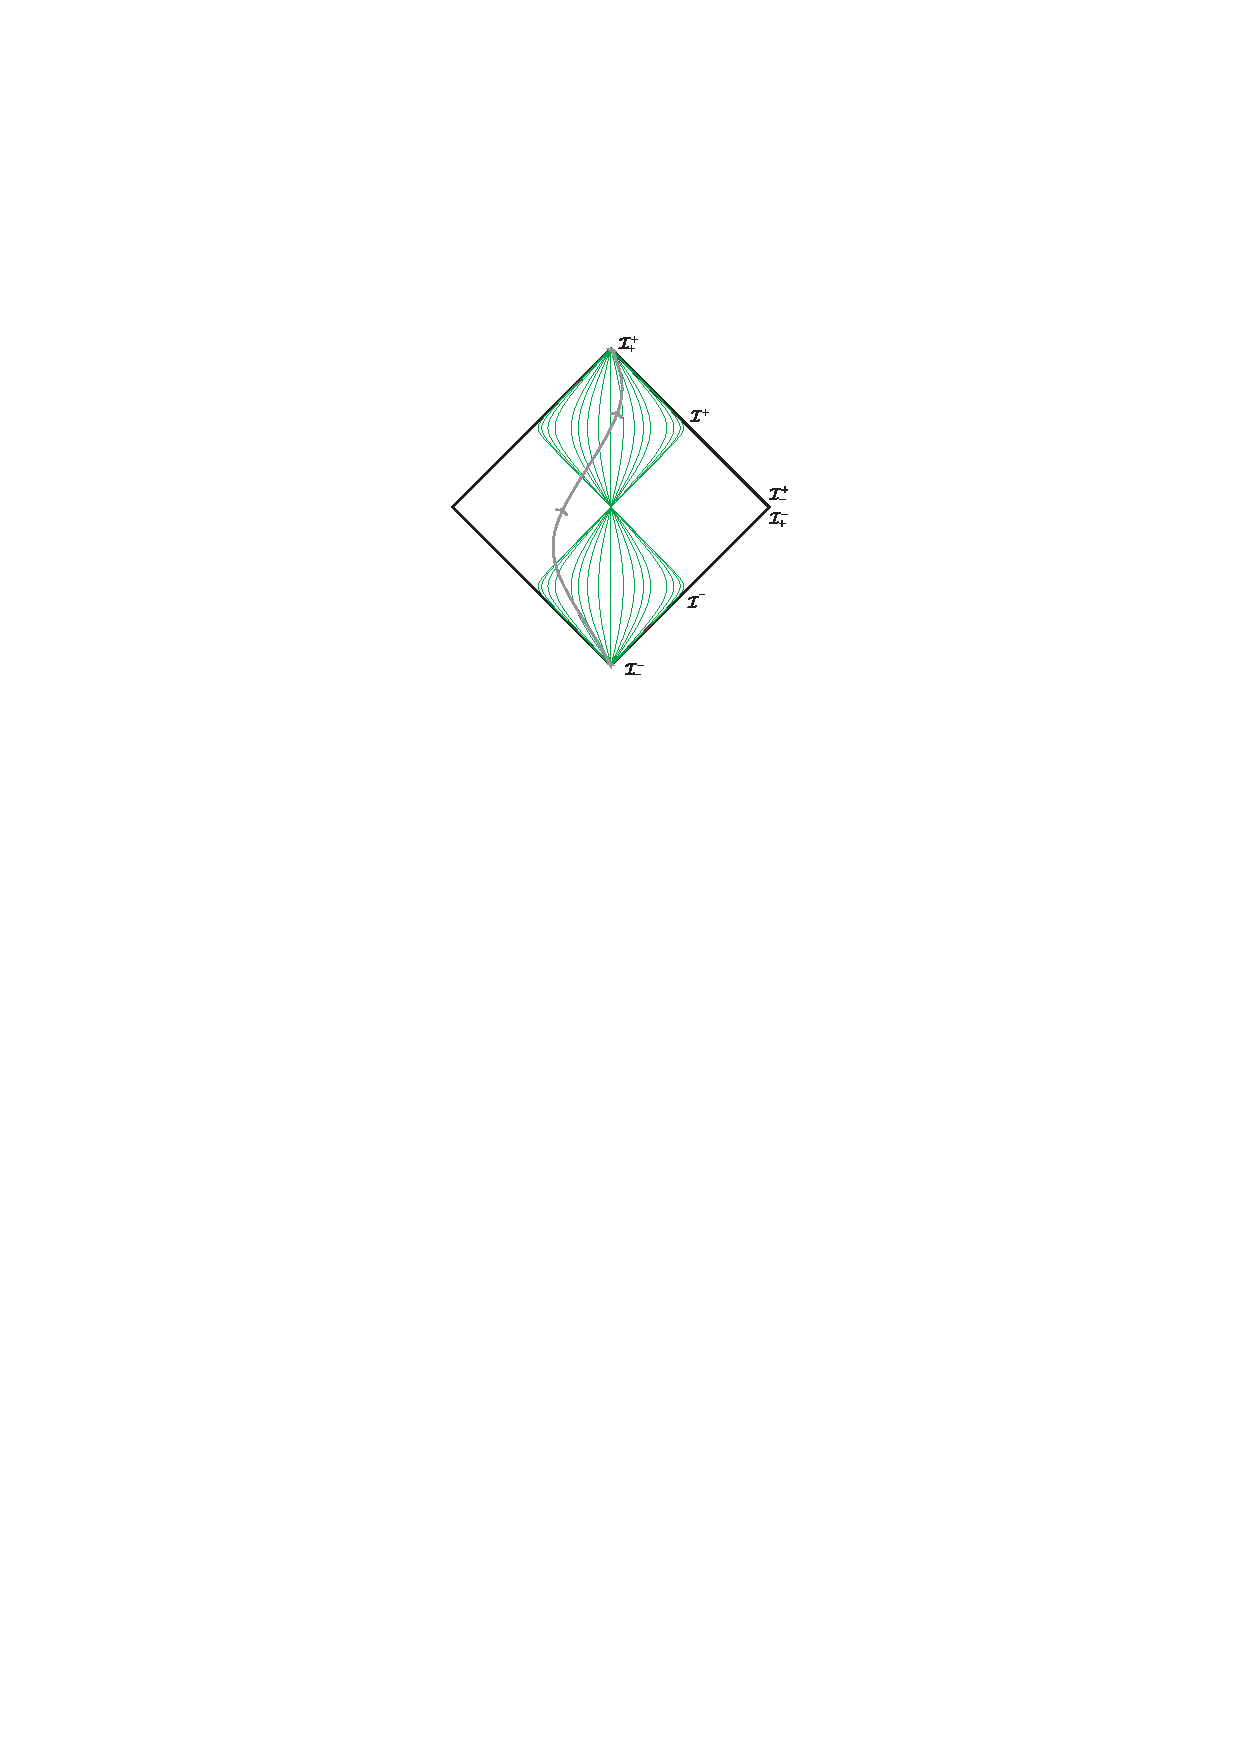
\includegraphics{figs/fig7.pdf}
	\caption{$\rho$ slices in Mink$_{4}$}
\end{figure}
考虑匀速运动的有质量粒子,$\vec{r}=\frac{\vec{p}}{E}t+\vec{\vec{r}_{0}}$:
\begin{equation}
	\begin{aligned}
		&\rho=\frac{r}{\sqrt{t^{2}-r^{2}}}=\frac{|\frac{1}{E}\vec{p}t+\vec{r}_{0}|}{\sqrt{t^{2}-\left(\frac{1}{E}\vec{p}t+\vec{r}_{0}\right)^{2}}}, \\
		&\tau=\sqrt{t^{2}-r^{2}}=\sqrt{t^{2}-\left(\frac{1}{E}\vec{p}t+\vec{r}_{0}\right)^{2}}, \\
		&\hat{x}=\frac{\vec{r}}{r}=\frac{\vec{p}t+E\vec{r}_{0}}{|\vec{p}t+E\vec{r}_{0}|}.
	\end{aligned}
\end{equation}
取$t\to\infty$的极限:
\begin{equation}
	\tau\to\frac{m}Et\to\infty,\quad\rho\to\frac{|\vec{p}|}m,\quad\hat{x}\to\hat{p}.
\end{equation}
可以看到粒子的世界线最终会趋近于某个$\rho$ slice,而且在$i^+$球上的方位也是确定的。这和前面$\mathcal{I}^+$上的情况完全相同,只不过那个时候是$\mathbb{R}\times \mathcal{S}^2$的结构,我们也是用粒子在哪个天球$(u)$以及在天球上的何处$(z,\bar z)$来标记粒子。现在的步骤就是写下辛形式进行量子化找到对易子。不难猜到最终的结果为:
\begin{equation}\label{guess}
	Q_{\varepsilon}^{+H}\left|\vec{p}\right>=Q\varepsilon\left(\frac{\left|\vec{p}\right|}{m},\hat{p}\right)\left|\vec{p}\right\rangle 
\end{equation}
与前面无质量的情况完全类似,只是这个时候large gauge $\varepsilon$不是boundary上的,而是bulk里的。但是这个结果并非显然,前面我们虽然是直接使用Noether定理“看”出来的,但更严谨的做法还是得去构造带电粒子的相空间辛形式,搞渐近分析和surface charges那一套。文献\cite{Campiglia:2015qka}对复标量场,也就是标量QED进行了仔细分析,稍微总结一下思路,首先是弯曲时空量子场论中算过自由标量场的模式展开,其和平直时空一样是傅里叶展式:\sn{Lecture\cite{Strominger:2017zoo}的习题里面讨论了这个问题,但讨论的是更为简单的$\phi=\phi^\dagger$的实标量场,而我们标量QED里面需要的是复标量场,这样才有$U(1)$对称性,参与耦合的$U(1)$流不等于0,所以下面我按照文献\cite{Campiglia:2015qka}的公式,顺着习题的思路进行了改写}
\begin{equation}
	\varphi(x)=\int\frac{d^3\vec{p}}{(2\pi)^32E_p}(b(\vec{p})e^{ip\cdot x}+d^\dagger(\vec{p})e^{-ip\cdot x})
\end{equation}
利用$\rho,\tau$可以将相因子写成:
\begin{equation}
	p\cdot x=\tau\Big[-\sqrt{p^2+m^2}\sqrt{1+\rho^2}+\rho\vec{p}\cdot\hat{x}\Big]\equiv-\tau f(\vec{p})
\end{equation}
类似于前面对光子的处理,我们感兴趣荷是在$|\tau|\to\infty$的柯西面上定义的,所以去考虑$\tau\to-\infty$附近的展开\sn{后面一律考虑$Q^+$,$\tau\to-\infty$对应的$Q^-$讨论类似}。利用鞍点近似,将$f(\vec{p})$在鞍点$\vec{p}=m\rho\hat x$附近进行展开:
\begin{equation}
	p\cdot x=-m\tau-\frac{\tau}{2}\mathcal{P}_{ij}(p_{i}-m\rho\hat{x}_{i})(p_{j}-m\rho\hat{x}_{j})+\mathcal{O}(p^{3})
\end{equation}
这里$\mathcal{P}_{ij}$是Hessian矩阵:
\begin{equation}
	\mathcal{P}_{ij}\equiv\left.\frac{\partial}{\partial p_i}\frac{\partial}{\partial p_j}f\right|_{\vec{p}=m\rho\hat{x}}=\frac{1}{m}\left[\delta_{ij}-\frac{\rho^2}{1+\rho^2}\hat{x}_i\hat{x}_j\right]
\end{equation}
代入$\varphi$的模式展开得到:\begin{margintable}\footnotesize 
	\begin{tabularx}{\marginparwidth}{|X}
		$\int_{-\infty}^{\infty}dxe^{ikx^2}=\sqrt{\frac{\pi}{k}}e^{i\pi/4}$\\
		$\det\mathcal{P}=\frac{1}{m^3(1+\rho^2)}$
	\end{tabularx}
\end{margintable}
\begin{equation}\label{26.14}
	\begin{aligned}
		\lim_{\tau\to+\infty}\varphi(x)=& \frac1{2m(2\pi)^3\sqrt{1+\rho^2}}\left[b(m\rho\hat{x})e^{-im\tau}\int d^3pe^{-i\frac\tau2{\mathcal P}_{ij}p_ip_j}\right.  \\
		&+d^{\dagger}(m\rho\hat{x})e^{im\tau}\left.\int d^{3}pe^{i\frac{\tau}{2}\mathcal{P}_{ij}p_{i}p_{j}}\right] \\
		=&\frac{\sqrt{\frac{(2\pi)^3}{\tau^3\det\mathcal{P}}}}{2m(2\pi)^3\sqrt{1+\rho^2}}\left[b(m\rho\hat{x})e^{-im\tau}e^{-3i\pi/4}+d^\dagger(m\rho\hat{x})e^{im\tau}e^{3i\pi/4}\right]\\
		=&\frac{\sqrt{m}}{2(2\pi\tau)^{3/2}}\left[b(m\rho\hat{x})e^{-im\tau}e^{-3i\pi/4}+d^\dagger(m\rho\hat{x})e^{im\tau}e^{3i\pi/4}\right]
	\end{aligned}
\end{equation}
现在选取用$\tau$分割的某个$\mathbb{H}_3$ Slice作为柯西面\sn{柯西面从几何上看一个重要的特性就是与所有粒子的世界线最终相交的类空曲面}。对应相空间辛形式为:\sn{这里$\mathbb{H}_3$表示$\tau=1$所对应的单位双曲面,$d^3V$是上面$SL(2,\mathbb{C})$不变的积分测度}
\begin{equation}
	\Omega_{\tau}=\int d^{3}V\tau^{3}\partial_{\tau}\delta\varphi\wedge\delta\varphi+h.c
\end{equation}
进一步选取$\tau\to\infty$对应的柯西面,这样就能使用\ref{26.14}进一步简化式子:
\begin{equation}
	\Omega_{\tau\to\infty}=-\frac{im^2}{2(2\pi)^3}\int d^3V\left(\delta b(m\rho\hat{x})\wedge\delta b^\dagger(m\rho\hat{x})+b\leftrightarrow d\right)
\end{equation}
这个辛形式得到的$b,b^\dagger$之间的对易关系与平直时空里的完全一致!
\begin{equation}
	\begin{aligned}
		\left[b(m\rho\hat{x}),b^\dagger(m\rho'\hat{x}')\right]&=\frac{2(2\pi)^3}{m^2}\delta(\rho-\rho')\delta^2(\hat{x}-\hat{x}')=(2\pi)^{3}(2\omega_{p})\delta^{3}(\vec{p}-\vec{p^{\prime}})
		&=\left[d(m\rho\hat{x}),d^\dagger(m\rho'\hat{x}')\right]
	\end{aligned}
\end{equation}
我们知道标量QED里面的$U(1)$流为:
\begin{equation}
	\mathcal{J}_\mu=ie\varphi(D_\mu\varphi)^\dagger+h.c.,\quad D_\mu\varphi\equiv\partial_\mu\varphi-ie{A}_\mu\varphi 
\end{equation}
现在hard charges就可以利用bulk里面的$\varepsilon$以及$\tau\to\infty$时的$U(1)$流来定义:
\begin{equation}
	Q_\varepsilon^{+H}=-\int_{\mathbb{H}_3}d^3V\varepsilon(\rho,\hat{x})j^\tau(\rho,\hat{x})
\end{equation}
其中:
\begin{equation}
	j^\tau(\rho,\hat{x})=\lim_{\tau\to\infty}\tau^3\mathcal{J}^\tau(\tau,\rho,\hat{x})=\frac{em^2}{2(2\pi)^3}(b(\rho,\hat{x})b^\dagger(\rho,\hat{x})-d(\rho,\hat{x})d^\dagger(\rho,\hat{x}))
\end{equation}
从物理上讲,我们可以认为这个荷由large gauge对hard粒子的作用生成,再利用$b,b^\dagger$之间的对易关系就可以得到\ref{guess}。

类似于\ref{eq:24.2},可以得到:\sn{注意这里不使用上标in,out来标记出入射,螺旋度、电荷、能量的大小用$h,Q,p^0$表示,那么出射粒子的物理量为$-h,-Q,-p^0$}
\begin{equation}
	\begin{aligned}
		\langle\mathrm{out}|Q_{\varepsilon}^{+}& =-2\int d^{2}w\partial_{\bar{w}}\varepsilon\langle\mathrm{out}|\partial_{w}N  \\
		&+\sum_{k\in\mathrm{massless}}Q_{k}\varepsilon(z_{k},\bar{z}_{k})\langle\mathrm{out}|+\sum_{k\in\mathrm{massive}}Q_{k}\varepsilon\left(\frac{|\vec{p}_{k}|}{m_{k}},\hat{p}_{k}\right)\langle\mathrm{out}|
	\end{aligned}
\end{equation}
Ward恒等式为:
\begin{equation}
\begin{aligned}
	&-2\int d^{2}w\partial_{\vec{w}}\varepsilon\partial_{w}\left\langle\mathrm{out}|\left[N(w,\bar{w})\mathcal{S}-\mathcal{S}N^{-}(w,\bar{w})\right]|\mathrm{in}\right\rangle  \\
	&=-\left[\sum_{k\in\mathrm{massless}}Q_{k}\varepsilon(z_{k},\bar{z}_{k})+\sum_{k\in\mathrm{massive}}Q_{k}\varepsilon\left(\frac{|\vec{p}_{k}|}{m_{k}},\hat{p}_{k}\right)\right]\langle\mathrm{out}|\mathcal{S}|\mathrm{in}\rangle
\end{aligned}
\end{equation}
取$\varepsilon(w,\bar{w})=\frac1{z-w}$,得到:
\begin{equation}
	\begin{aligned}
		\frac{\sqrt{2}}{1+z\bar{z}}&\lim_{\omega\to0^{+}}\left[\omega\left\langle\mathrm{out}\right|a_{+}\big(\omega\hat{x}(z,\bar{z})\big)\mathcal{S}\left|\mathrm{in}\right\rangle\right] \\
		&=e\left[\sum_{k\in\text{massless}}\frac{Q_k}{z-z_k}+\sum_{k\in\text{massive}}Q_k\varepsilon\left(\frac{|\vec{p}_k|}{m_k},\hat{p}_k\right)\right]\langle\text{out}|\mathcal{S}|\text{in}\rangle
	\end{aligned}
\end{equation}
利用格林函数的又双叒叕一种表达式:
\begin{equation}
	G\left(\frac{|\vec{p_k}|}m,\hat{p}_k;w,\bar{w}\right)=\frac{1}{2\pi}\partial_{\bar{w}}\left[\frac{\sqrt{2}}{1+w\bar{w}}\frac{p_k\cdot\epsilon^+}{p_k\cdot\hat{q}}\right]
\end{equation}
得到:\sn{分部积分加上$$\partial_{\bar{z}}\frac{1}{z-w}=2\pi\delta^2(z-w)$$}
\begin{equation}
	\varepsilon\left(\frac{|\vec{p_k}|}{m},\hat{p}_k\right)=\frac{\sqrt{2}}{1+z\bar{z}}\frac{p_k\cdot\epsilon^+}{p_k\cdot\hat{q}}
\end{equation}
代回到Ward恒等式就再次得到了软定理!
\section{Further Progress}
\subsection{Subleading order}
本节集中处理无质量标量QED中的软定理次领头阶贡献与Ward恒等式的对应,文献\cite{Lysov:2014csa}首先进行了处理,而且引言部分总结了天球物理上的诸多疑点,但注意这已经是十年前的文献了,而且文章的处理思路与现在的处理方法是顺序相反的,并非先利用对径认同找守恒荷。文献\cite{Campiglia:2016hvg}对此进行了补充。
\subsection{Magnetic monopole}
Strominger认为,前面对软定理的推导是在微扰理论的框架下进行的(使用了费曼图就肯定是在研究微扰场论了),但是QED本身由于朗道极点的存在就必然是UV不完备的,所以要计算软定理领头阶的非微扰贡献,求助于构造一个非微扰的QED是徒劳。不过Strominger认为有磁荷的QED或许能解决这个问题\cite{Strominger:2015bla}。

磁荷同样可以和软光子相互作用,磁荷对软定理领头阶的修正可以完全地通过电磁对偶的手段非常简洁地建立起来。
\begin{equation}
	\tilde{F}=-\frac{2\pi}{e^{2}}*F,\quad\tilde{e}=\frac{2\pi}{e},\quad\tilde{Q}_{k}=\frac{1}{\tilde{e}^{2}}\int_{S_{k}^{2}}*\tilde{F}=M_{k},\quad\tilde{M}_{k}=\frac{1}{2\pi}\int_{S_{k}^{2}}\tilde{F}=-Q_{k}
\end{equation}
这里$S_k^2$表示包围第$k$个电/磁荷的球面。通过上面的对偶变换,我们建立了$\left(\tilde{Q},\tilde{M}\right)\leftrightarrow\left(M,-Q\right)$的对应,从数学结构上看,磁荷和电荷是完全类似的。注意,我们这里做的操作只是数学上的换元而已,方便我们看出背后的数学结构,并未事先假定电磁之间存在某种对偶。那么类似的磁荷也会和规范场$\tilde{A}$相互作用:
\begin{align}
	F=dA,\quad A=e\varepsilon_\alpha \mathrm{e}^{iq\cdot x}\\
	\tilde{F}=\mathrm{d}\tilde{A}=-\frac{2\pi}{e^2}*\mathrm{d}A,\quad \tilde{A}=\tilde{e}\tilde{\varepsilon}_\alpha \mathrm{e}^{iq\cdot x}
\end{align}
所以磁荷那部分的修正只需要做替换$A\mapsto \tilde A,e\mapsto \tilde e,\varepsilon_\alpha\mapsto \tilde{\varepsilon}_\alpha$即可得到。
\begin{equation}
	S_0^\alpha=\sum_k\eta_k\frac{eQ_kp_k\cdot\varepsilon^\alpha}{q\cdot p_k}\to \sum_k\eta_k\frac{p_k\cdot(Q_ke\varepsilon^\alpha+M_k\tilde{e}\tilde{\varepsilon}^\alpha)}{q\cdot p_k}
\end{equation}
这个式子可以进一步化简,将前面的对偶推到天球上去看:
\begin{equation}
	\tilde{F}_{z\bar{z}}^{(0)}=\frac{2\pi i}{e^2}\gamma_{z\bar{z}}F_{ru}^{(2)},\quad\tilde{F}_{ru}^{(2)}=\frac{2\pi i}{e^2}\gamma^{z\bar{z}}F_{z\bar{z}}^{(0)},\quad\tilde{F}_{uz}^{(0)}=\frac{2\pi i}{e^2}F_{uz}^{(0)}
\end{equation}
最后一个式子说明:
\begin{equation}
	\tilde{A}_z^{(0)}=\frac{2\pi i}{e^2}A_z^{(0)}
\end{equation}
同时也给出了$\varepsilon_\alpha$和$\tilde{\varepsilon}_\alpha$之间的比例系数。软定理(领头阶)最终化简为:
\begin{equation}\label{28.7}
	\boxed{S_0^\pm=\sum_k\eta_k\frac{(eQ_k\pm\frac{2\pi i}{e}M_k)p_k\cdot\varepsilon^\pm}{q\cdot p_k}}
\end{equation}
Strominger认为这应当是考虑了非微扰效应之后的软定理领头阶的精确表达式。类似\ref{24.12},磁荷这边也有:
\begin{equation}
	F_{z\bar{z}}^{(0)}|_{\mathcal I_{-}^{+}}=-F_{z\bar{z}}^{(0)}|_{\mathcal I_{+}^{-}}
\end{equation}
负号是因为方向角选取对径认同,所以$\partial_z\leftrightarrow-\partial z$。前面不考虑磁荷时,认为天球上$F_{z\bar z}-0$。这样就可以利用对径认同的天球上的任意函数$\varepsilon(z,\bar z)$定义守恒的荷:
\begin{align}
	&\tilde{Q}_{\varepsilon}^{+}=\frac{1}{2\pi}\int_{\mathcal I_{-}^{+}}\varepsilon F=\frac{i}{2\pi}\int_{\mathcal I_{-}^{+}}d^{2}z\varepsilon F_{z\bar{z}}^{(0)}\\
	&\tilde{Q}_{\varepsilon}^{-}=-\frac{1}{2\pi}\int_{\mathcal I_{+}^{-}}\varepsilon F=-\frac{i}{2\pi}\int_{\mathcal I_{+}^{-}}d^{2}z\varepsilon F_{z\bar{z}}^{(0)}
\end{align}
\begin{equation}
	\boxed{
		\tilde{Q}_{\varepsilon}^+=\tilde{Q}_{\varepsilon}^-
	}
\end{equation}
再次得到了无穷多个守恒荷,对应的又是何种对称性呢?或许我们可以完全类似于电荷认为它对应磁荷的large gauge symmetries:
\begin{equation}\label{conjecture1}
	\tilde{\delta}_\varepsilon\tilde{A}_z^{(0)}=\partial_z\varepsilon
\end{equation}
利用$A$可以表达为:
\begin{equation}
	\tilde\delta_{\varepsilon}A_{z}^{(0)}=-\frac{ie^{2}}{2\pi}\partial_{z}\varepsilon 
\end{equation}
从$A_z$这边看,加入磁荷后相当于原先的$U(1)$ large gauge 变成了一个\textbf{复化}之后的large gauge,对应的守恒荷也复化了。

按理说现在要做的事情就是重复前面模式展开、协变相空间量子化那一套去证明Ward恒等式和\ref{28.7}之间的等价性,\cite{Strominger:2015bla}也这么去做了,但是却存在一些非常大的conjecture。首先认为$\tilde{Q}^\pm$由\ref{conjecture1}生成就是一个猜想,$\tilde{A}$确实存在\ref{conjecture1}这样的large gauge,但是最终这证明$\tilde{Q}^\pm$是其生成元需要构造协变相空间的量子化从而计算对易子。这就导出了另外一个conjecture,我们并不知道磁荷的辛形式如何去构造,而且前面推导电荷那边辛形式非常重要的一个边界条件是假定没有磁荷,加入磁荷之后辛形式如何修改还不清楚,我们只能认为加入磁荷后$Q^\pm$依旧由电荷的large gauge生成。文献\cite{Strominger:2015bla}就是在这些假定下去做的。

另外一个比较重要的点,电荷那边的large gauge是$U(1)$ gauge的一个子群,常说$U(1)$ gauge不是symmetry,只是冗余自由度,要么没有守恒荷,要么构建出的守恒荷其实不守恒\sn{我们讲对称性,首先要可以从Noether定理导出可观测的守恒荷,而且有相应的对物理态的对称变换。global的$U(1)$对称性确实non-trivial,是真正的symmetry,对应电荷守恒,这其实上无穷远处不归零已经有large gauge的影子了,但是local $U(1)$ 是trivial的,它导出电荷守恒并非是Noether定理的结论(回忆Nother定理的那些标记连续对称性的参数是global的而不是local的)。},这些“symmetry”是trivial的,只是redundancy,并非渐近对称性,我们可以把通常所说的$U(1)$ gauge称为“bulk gauge”,而天球上的large gauge是真正的渐近对称性。对于QED的情况,large gauge是bulk gauge的子群,或者说非平庸的子群,但是磁荷这边就不一样了,上面通过对偶看出来的渐近对称性并不能看成bulk gauge的子群,毕竟都出现复化跑出$U(1)$了,所以通过这点可以看出,\textbf{并不是所有的渐近对称性都可以看作是bulk里的对称性的子群}
\subsection{Non-Abelian gauge theory}
\subsection{Higher dimensions}
\subsection{$\mathcal{N}=1$ Super Symmetry}


